% Preview source code

%% LyX 2.3.0 created this file.  For more info, see http://www.lyx.org/.
%% Do not edit unless you really know what you are doing.
\documentclass[twocolumn,journal]{IEEEtran}
\usepackage[T1]{fontenc}
\usepackage[utf8]{inputenc}
\usepackage{calc}
\usepackage{graphicx}
\usepackage[unicode=true,
 bookmarks=true,bookmarksnumbered=true,bookmarksopen=true,bookmarksopenlevel=1,
 breaklinks=false,pdfborder={0 0 0},pdfborderstyle={},backref=false,colorlinks=false]
 {hyperref}

\hypersetup{pdftitle={Your Title},
 pdfauthor={Your Name},
 pdfpagelayout=OneColumn, pdfnewwindow=true, pdfstartview=XYZ, plainpages=false}


 \makeatletter
 \def\endthebibliography{%
   \def\@noitemerr{\@latex@warning{Empty `thebibliography' environment}}%
   \endlist
 }
 \makeatother

 \usepackage[round, numbers]{natbib}
 \bibliographystyle{unsrtnat}

\makeatletter
%%%%%%%%%%%%%%%%%%%%%%%%%%%%%% Textclass specific LaTeX commands.
% protect \markboth against an old bug reintroduced in babel >= 3.8g
\let\oldforeign@language\foreign@language
\DeclareRobustCommand{\foreign@language}[1]{%
  \lowercase{\oldforeign@language{#1}}}

%%%%%%%%%%%%%%%%%%%%%%%%%%%%%% User specified LaTeX commands.
% for subfigures/subtables
\usepackage[caption=false,font=footnotesize]{subfig}


\usepackage{amsmath,amssymb}
\usepackage{amsthm}
\newtheorem{theorem}{Theorem}
\newtheorem*{cor}{Corollary}
\newtheorem{lemma}[theorem]{Lemma}
\DeclareMathOperator\erfc{erfc}
\DeclareMathOperator\erf{erf}



\@ifundefined{showcaptionsetup}{}{%
 \PassOptionsToPackage{caption=false}{subfig}}
\usepackage{subfig}
\makeatother

\setcitestyle{square}

\begin{document}

\title{Autocorrelation in Sparse Distributed Memory}

\author{Marcelo S. Brogliato,~\IEEEmembership{Member,~IEEE,} and Alexandre
Linhares, \IEEEmembership{Member,~IEEE,}\thanks{Dr. Brogliato is with sdm.ai and with Behavioral and Decision Sciences,
EBAPE, Fundação Getulio Vargas, Rio de Janeiro, Brazil, e-mail: \protect\href{http://msbrogli@sdm.ai}{msbrogli@sdm.ai}.}\thanks{Dr. Linhares is with sdm.ai and with Behavioral and Decision Sciences,
EBAPE, Fundação Getulio Vargas, Rio de Janeiro, Brazil, e-mail: \protect\href{http://linhares@sdm.ai}{linhares@sdm.ai}.}}

\markboth{Working Paper}{Brogliato and Linhares: Autocorrelation in SDM}

\IEEEpubid{0000\textendash 0000/00\$00.00~\copyright~2012 IEEE}
\maketitle






\begin{abstract}
Sparse Distributed Memory (SDM) is a neuroscientific and psychologically
plausible model of human memory. In this paper we present an anomaly
between its previously theoretized behavior and its actual behavior,
and demonstrate that this anomaly is due to the autocorrelation involved
in the model. Our findings have systemwide implications for those
willing to implement and apply SDM in computational intelligence settings.
\end{abstract}

\begin{IEEEkeywords}
Sparse Distributed Memory, Autocorrelation, Theoretical Neuroscience, Memory,
Systemwide properties.
\end{IEEEkeywords}


\IEEEpeerreviewmaketitle{}






\section{Introduction}

\IEEEPARstart{S}{parse distributed memory} (SDM) \citep{Kanerva1988} (see also \citep{denning_sparse_1989,  flynn_sparse_1989, kanerva_sparse_1993, kanerva_parallel_1985, goos_binary_1996, kanerva_hyperdimensional_2009,  keeler_comparison_1988, rwcp_fully_1997, marinaro_spatter_1994, sahlgren_permutations_nodate, uesaka_foundations_2001}) is a mathematical model of long-term memory that has a number of neuroscientific and psychologically plausible dynamics. This model is used in all sort of applications due to its incredible ability to closely reflect the human capacity to remember past experiences from the subtlest of clues. Applications range from call admission control \citep{kwon_atm_1998, hee-yong_kwon_atm_1997}, to behavior-based robotics \citep{Rajesh1998, mendes2008robot, jockel_sparse_2009}, to noise filtering \citep{meng_modified_2009}, etc.


\begin{figure}[h!]
  \centering
  \subfloat[$Q_3$]{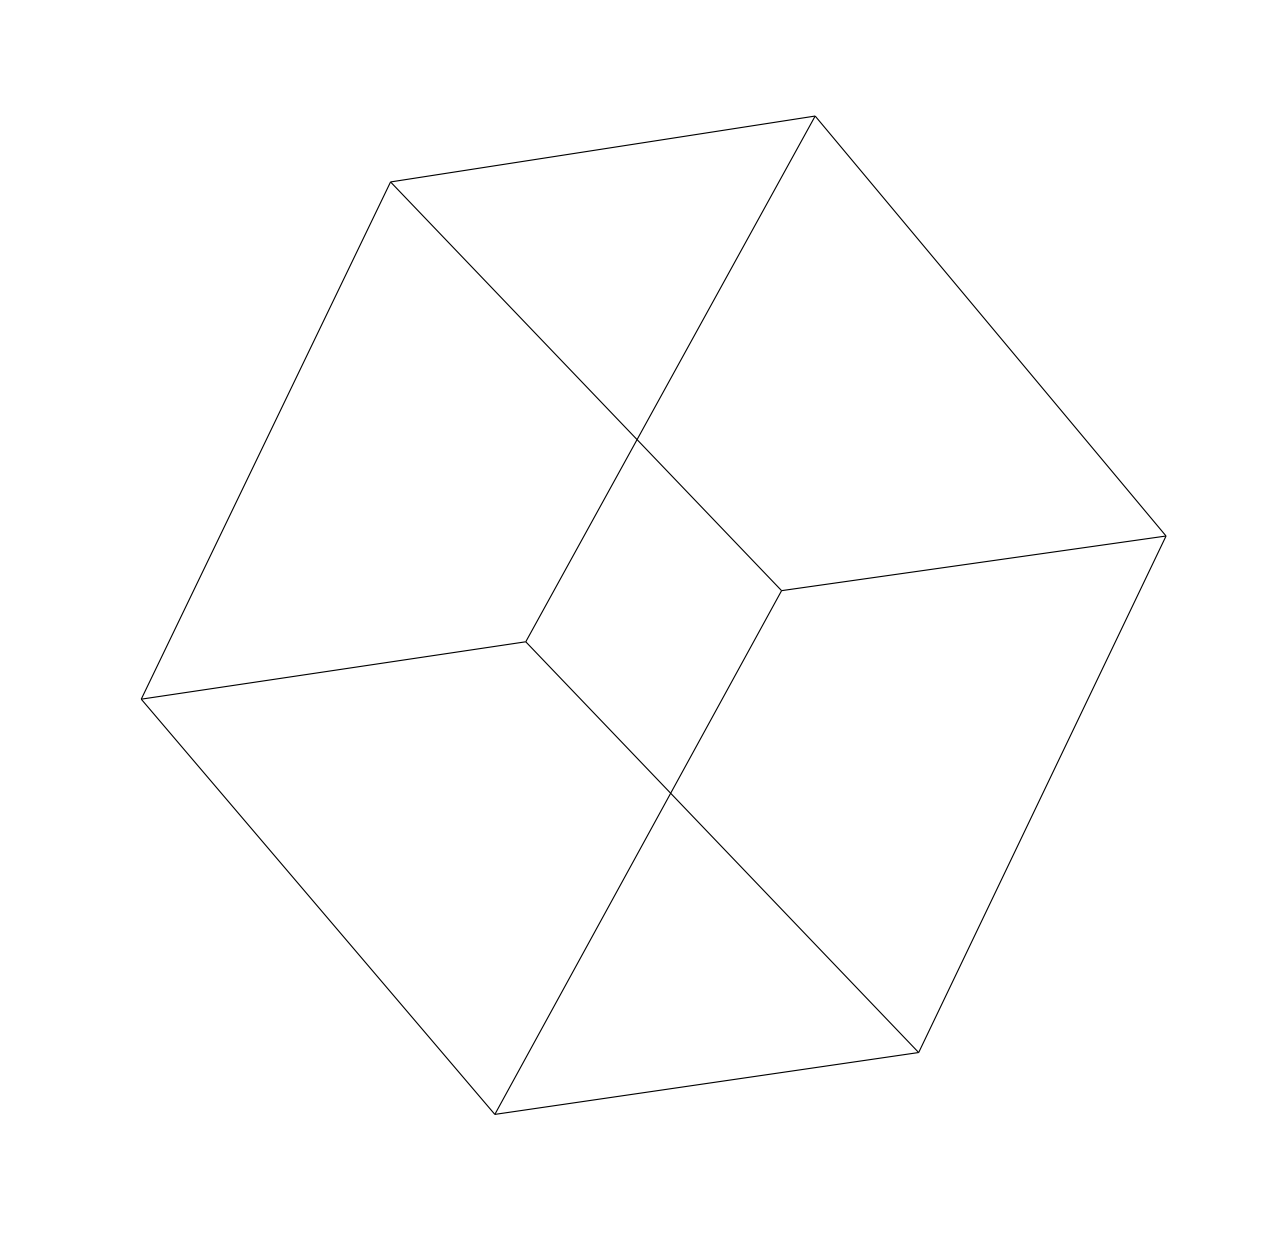
\includegraphics[width=0.4\columnwidth]{./images02/new-images/qn3.png}}
  \subfloat[$Q_7$]{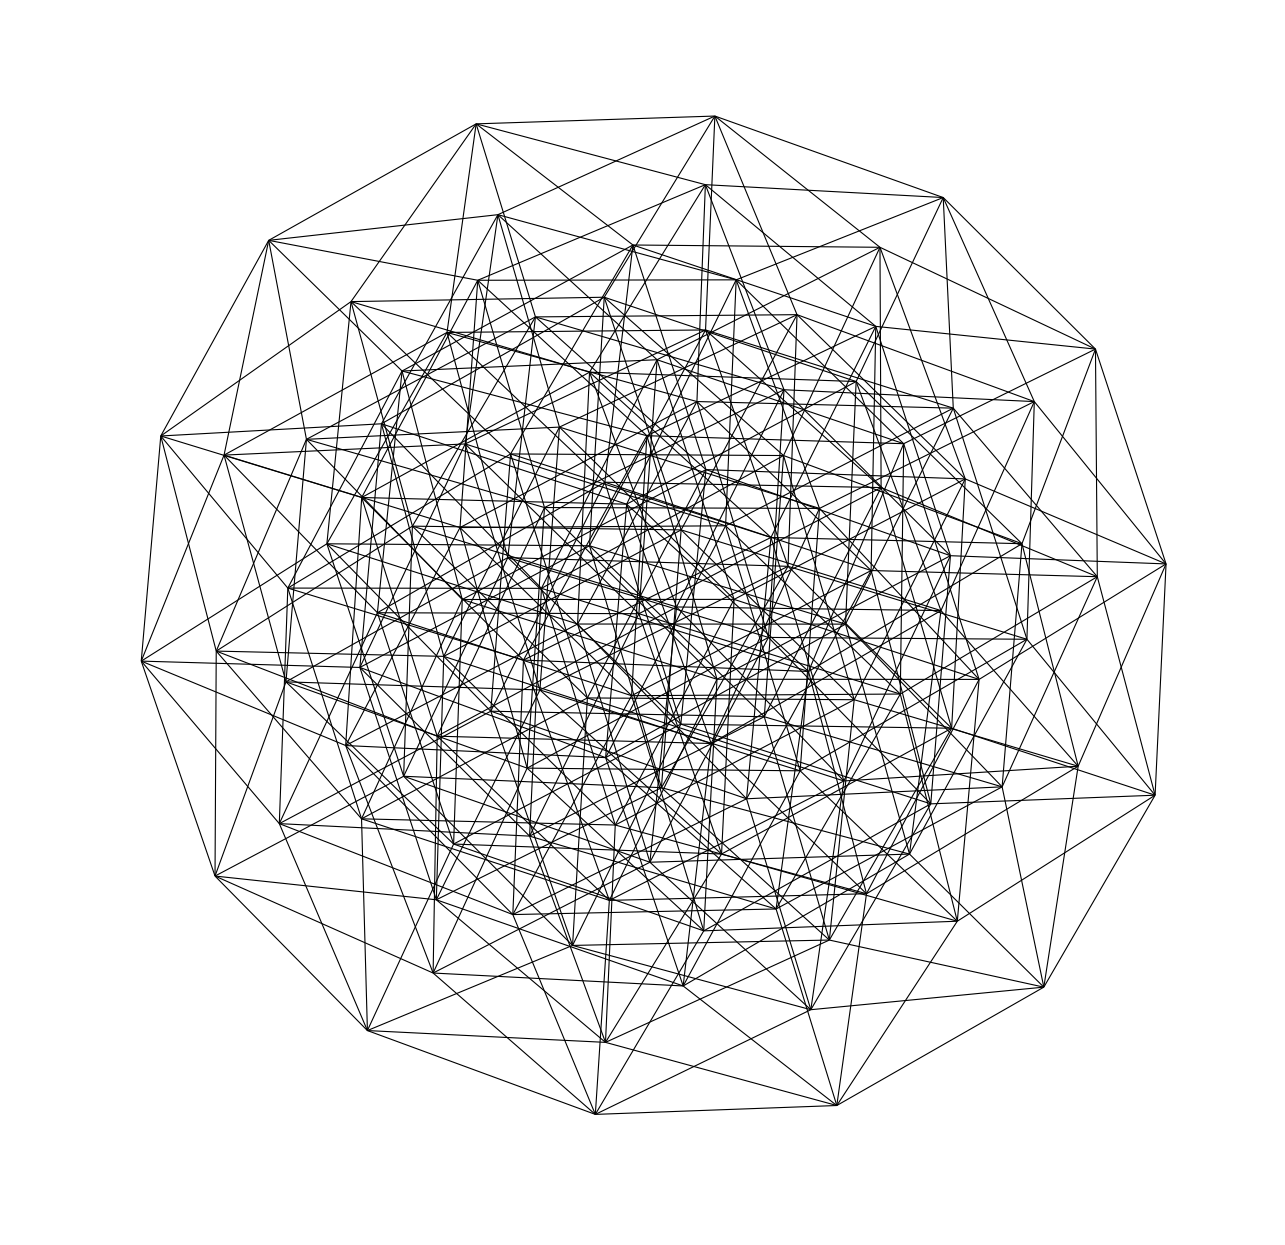
\includegraphics[width=0.4\columnwidth]{./images02/new-images/qn7.png}}

  \subfloat[$Q_{10}$]{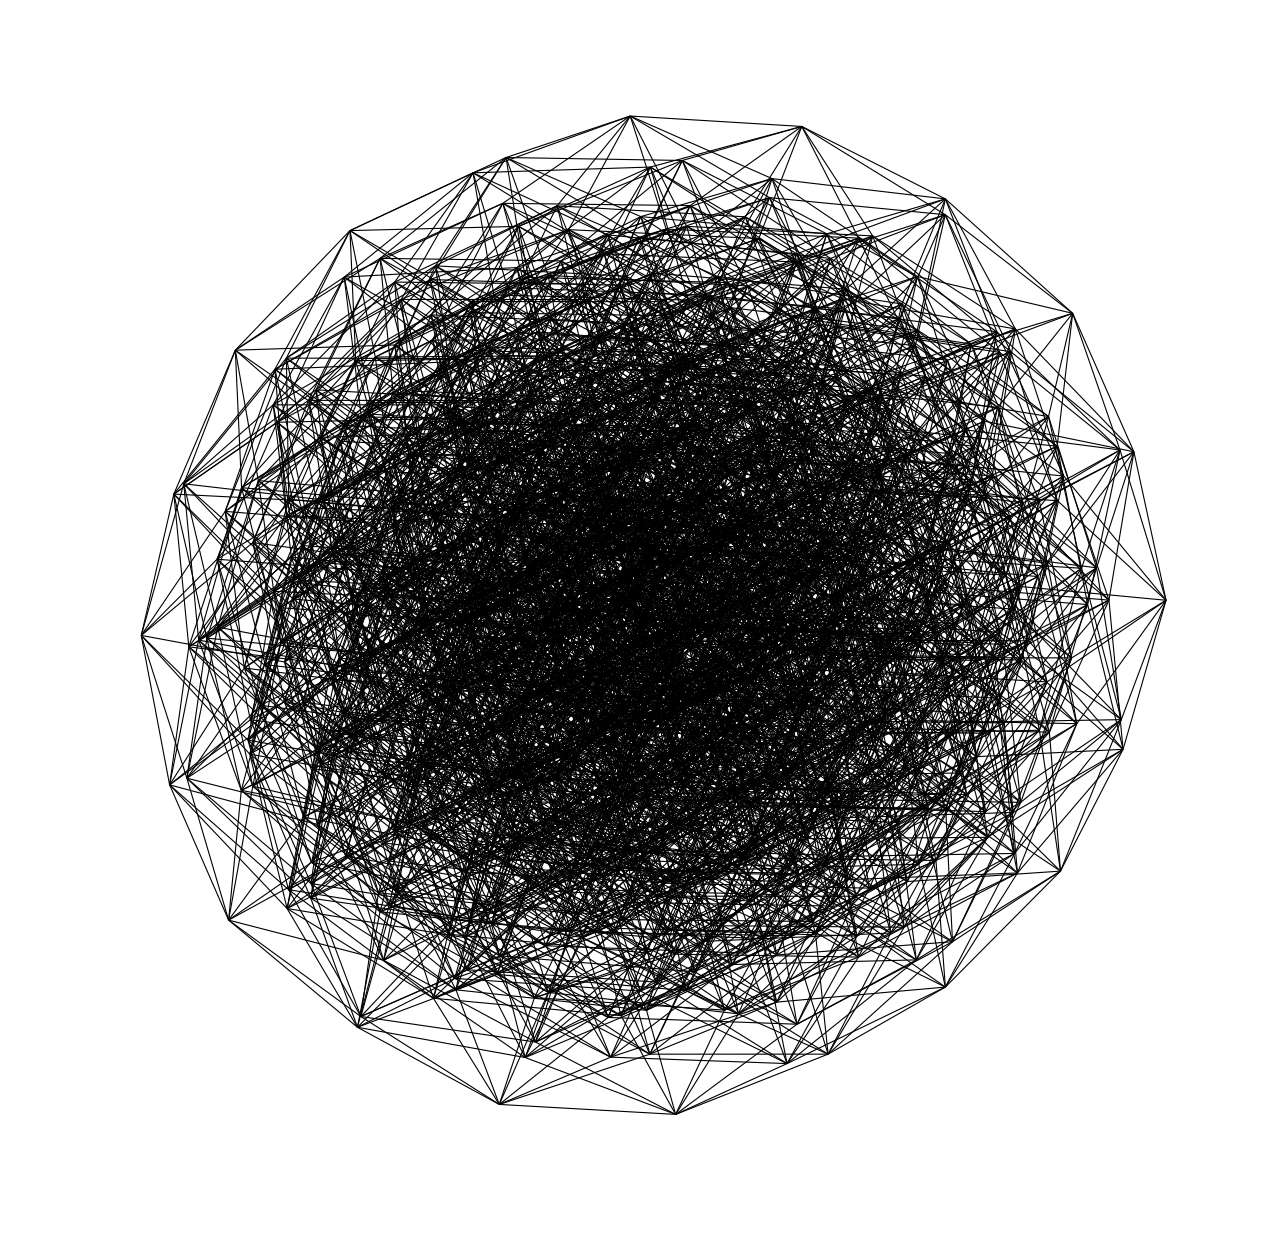
\includegraphics[width=\columnwidth]{./images02/new-images/qn10.png}}
  \caption{Kanerva models the space of \emph{possible incoming neural signals} as an $n$-dimensional \emph{hypercube}, or $Q_n$.  Here we have $Q_n$, for $n \in$ \{3, 7, 10\}. Each node corresponds to a bitstring in $\{0,1\}^n$, and two nodes are linked iff the bitstrings differ by a single dimension.  A number of observations can be made here. First, the number of nodes grows as $O(2^n)$; which makes the space rapidly intractable. Another interesting observation is that most of the space lies `at the core' of the hypercube, at a distance of around $n/2$ from any given vantage point.\label{hypercubes}}
\end{figure}


\subsection{Review of the model}

IN SDM, the data --- and address space on which it is stored --- are represented by large \emph{bitstrings}. The \emph{Hamming distance} provides comparisons between bitstrings and is used as a metric for the system. This space is also called the \emph{hypercube graph}, or $Q_n$, as in Figure \ref{hypercubes}. For a fixed $n \in \mathbb{Z}$, the graph $G = (V, E)$, in which $v \in V$ iff there is a bijective function $b: V\to \{0,1\}^n$ and $(v_i, v_j) \in E$ iff $H(b(v_i), b(v_j))=1$, where $H$ is the Hamming distance. That is, $n$-sized bitstrings correspond to nodes, and edges exist between nodes $iff$ they flip a single bit.  Though Kanerva has derived many combinatorial properties of the space, additional results have been found by the graph-theoretical community: it is a bipartite graph with chromatic number 2, and it is planar only if $n\le3$. The proofs, though elementary, illuminate some of its properties:  vertices connect bitstrings with an even number of 1's with bitstrings with an odd number of 1's, therefore (i) it is \emph{bipartite} and (ii) it \emph{may be colored with two colors}.  As for planarity, the case $n=3$ is the largest planar one.  A good survey is provided by \citep{harary1988survey} --- and some interesting results may be found in \citep{foldes_characterization_1977, wagner_embedding_1990, laborde_another_1982, ruskey_combinatorial_2003}.




Unlike traditional memory used by computers, SDM performs read and write operations in a multitude of addresses, also called neurons.  That is, the data is not written, or it is not read in a single address spot, but in many addresses. These are called activated addresses, or activated neurons.

The activation of addresses takes place according to their distances from the datum. Suppose one is writing datum $\eta$ at address $\xi$, then all addresses inside a circle with center $\xi$ and radius $r$ are activated. So, $\eta$ will be stored in all these activated addresses, which are around address $\xi$, such as in Figure \ref{fig-addresses-inside-access-radius}.  An address $\xi'$ is inside the circle if its Hamming distance to the center $\xi$ is less than or equal to the radius $r$, i.e. $distance(\xi,\xi')\leq r$.

\begin{figure}[!htb]
\centering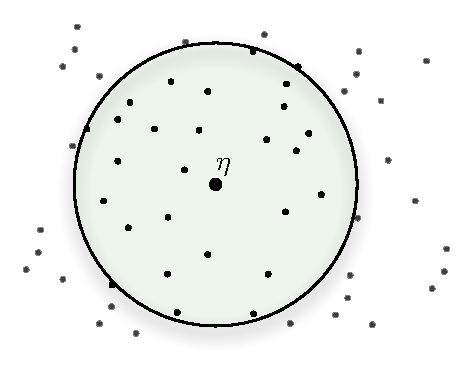
\includegraphics[scale=0.75]{./images02/p_circle_r.pdf}

\caption{Activated addresses inside access \protect \\
radius $r$ around the center address.\label{fig-addresses-inside-access-radius}}
\end{figure}



Every write or read in SDM memory activates a number of addresses with close distance.  The data is written in these activated addresses or read from them.  These issues will be addressed in due detail further on, but a major difference from a traditional computer memory is that the data are always stored and retrieved in a multitude of addresses. This way SDM memory has robustness against loss of addresses (e.g., death of a neuron).

In traditional memory, each datum is stored in an address and every lookup of a specific datum requires a search through the memory. In spite of computer scientists having developed beautiful algorithms to perform fast searches, almost all of them do a precise search. That is, if you have an imprecise clue of what you need, these algorithms will simply fail.

In SDM, the data space is the same as the address space, which amounts to a vectorial, binary space, that is, a $\{0,1\}^{n}$ space. This way, the addresses where the data will be written are the same as the data themselves. For example, the datum $\eta=00101_{b}\in\{0,1\}^{5}$ will be written to the address $\xi=\eta=00101_{b}$. If one chooses a radius of 1, the SDM will activate all addresses one bit away or less from the center address. So, the datum $00101_{b}$ will be written to the addresses $00101_{b}$, $10101_{b}$, $01101_{b}$, $00001_{b}$, $00111_{b}$, and $00100_{b}$.

In this case, when one needs to retrieve the data, one could have an imprecise cue at most one bit away from $\eta$, since all addresses one bit away have $\eta$ stored in themselves.  Extending this train of thought for larger dimensions and radius, exponential numbers of addresses are activated and one can see why SDM is a distributed memory.

When reading a cue $\eta_{x}$ that is $x$ bits away from $\eta$, the cue shares many addresses with $\eta$. The number of shared addresses decreases as the cue's distance to $\eta$ increases, in other words, as $x$ increases. This is shown in Figure \ref{fig-shared-addresses}.  The target datum $\eta$ was written in all shared addresses, thus they will bias the read output in the direction of $\eta$. If the cue is sufficiently near the target datum $\eta$, the read output will be closer to $\eta$ than $\eta_{x}$ was. Repeating the read operation increasingly gets results closer to $\eta$, until it is precisely the same. So, it may be necessary to perform more than one read operation to converge to the target data $\eta$.

\begin{figure}[!htb]
\centering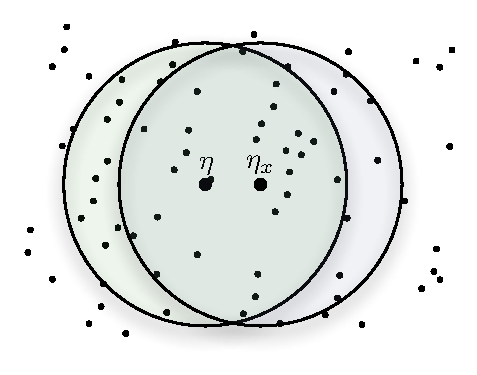
\includegraphics[scale=0.75]{./images02/p1_inter_p2.pdf}

\caption{Shared addresses between the \protect \\
target datum $\eta$ and the cue $\eta_{x}$. \label{fig-shared-addresses}}
\end{figure}


The addresses of the $\{0,1\}^{n}$ space grow exponentially with the number of dimensions $n$, i.e., $N=2^{n}$. For $n=100$ we have $N\approx10^{30}$, which is incredibly large when related to computer memory. Furthermore, \citep{Kanerva1988} suggests $n$ between 100 and 10,000.  To solve the feasibility problem of implementing this memory, Kanerva made a random sample of $\{0,1\}^{n}$, in his work, having $N'$ elements. All these addresses in the sample are called hard locations. Other elements of $\{0,1\}^{n}$, not in $N'$, are called virtual neurons. This is represented in Figure \ref{fig-hardlocations}.  All properties of reading and write operations presented before remain valid but limited to hard locations. Kanerva suggests taking a sample of about one million hard locations.

Using this sample of binary space, our data space does not exist completely.  That is, the binary space has $2^{n}$ addresses, but the memory is far away from having these addresses available. In fact, only a fraction of this vectorial space is actually instantiated. Following Kanerva's suggestion of one million hard locations, for $n=100$, only $100\cdot10^{6}/2^{100}=7\cdot10^{-23}$ percent of the whole space exists, and for $n=1,000$ only $100\cdot10^{6}/2^{1000}=7\cdot10^{-294}$ percent.

Kanerva also suggests the selection of a radius that will activate, on average, one-thousandth of the sample, which is 1,000 hard locations for a sample of one million addresses. In order to achieve his suggestion, a 1,000-dimension memory uses an access radius $r=451$, and a 256-dimensional memory, $r=103$. We think that a 256-dimensional memory may be important because it presents conformity to Miller's magic number \citep{Linhares2011}.

\begin{figure}[!htb]
\centering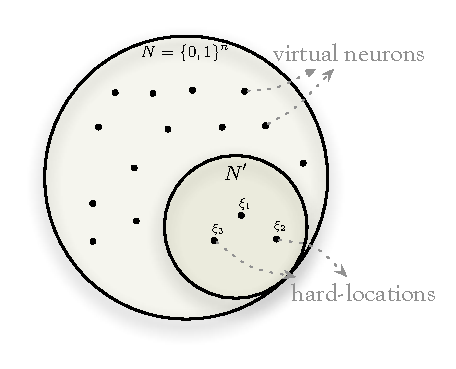
\includegraphics[scale=0.75]{./images02/hardlocations.pdf}

\caption{Hard-locations randomly sampled from binary space.\label{fig-hardlocations}}
\end{figure}


Since a cue $\eta_{x}$ near the target bitstring $\eta$ shares many hard locations with $\eta$, SDM can retrieve data from imprecise cues. Despite this feature, it is very important to know how imprecise this cue could be while still giving accurate results. What is the maximum distance from our cue to the original data that still retrieves the right answer? An interesting approach is to perform a read operation with a cue $\eta_{x}$, that is $x$ bits away from the target $\eta$.  Then measure the distance from the read output and $\eta$. If this distance is smaller than $x$ we are converging. Convergence is simple to handle, just read again and again, until it converges to the target $\eta$. If this distance is greater than $x$ we are diverging.   Finally, if this distance equals $x$ we are in a tip-of-the-tongue process.  A tip-of-the-tongue psychologically happens when you know that you know, but you can't say what exactly it is. In SDM mathematical model, a tip-of-the-tongue process takes infinite time to converge. \citet{Kanerva1988} called this $x$ distance, where the read's output averages $x$, the critical distance. Intuitively, it is the distance from which smaller distances converge and greater distances diverge. In Figure \ref{fig-p1-p2-iterative-read}, the circle has radius equal to the critical distance and every $\eta_{x}$ inside the circle should converge.  The figure also shows convergence in four readings.

\begin{figure}[!htb]
\centering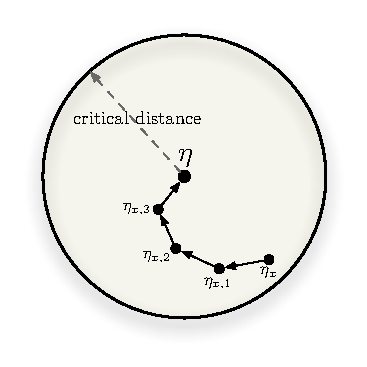
\includegraphics[scale=0.75]{./images02/p1_p2_iter_read.pdf}

\caption{In this example, four iterative readings were\protect \\
required to converge from $\eta_{x}$ to $\eta$.\label{fig-p1-p2-iterative-read}}
\end{figure}


The $\{0,1\}^{n}$ space has $N=2^{n}$ locations from which we instantiate $N'$ samples. Each location in our sample is called a hard location.  On these hard locations, we do operations of read and write. One of the insights of SDM is exactly the way we read and write: using data as addresses in a distributed fashion. Each datum $\eta$ is written in every activated hard location inside the access radius centered on the address, that equals datum, $\xi=\eta$. Kanerva suggested using an access radius $r$ having about one-thousandth of $N'$.  As an imprecise cue $\eta_{x}$ shares hard locations with the target bitstring $\eta,$ it is possible to retrieve $\eta$ correctly. (Actually, probably more than one read is necessary to retrieve exactly $\eta.)$.  Moreover, if some neurons are lost, only a fraction of the datum is lost and it is possible that the memory can still retrieve the right datum.

A random bitstring is generated with equal probability of $0$'s and $1$'s for each bit. One can readily see that the average distance between two random bitstrings follows the binomial distribution with mean $n/2$ and standard deviation $\sqrt{n/4}$. For a large $n$, most of the space lies close to the mean and has fewer shared hard locations.  As two bitstrings with distance far from $n/2$ are very improbable, \citet{Kanerva1988} defined that two bitstrings are orthogonal when their distance is $n/2$.

The write operation needs to store, for each dimension bit which happened more ($0$'s or $1$'s). This way, each hard location has $n$ counters, one for each dimension. The counter is incremented for each bit $1$ and decremented for each bit $0$. Thus, if the counter is positive, there have been more $1$'s than $0$'s, if the counter is negative, there have been more $0$'s than $1$'s, and if the counter is zero, there have been an equal number of $1$'s and $0$'s.

The read is performed polling each activated hard location and statistically choosing the most written bit for each dimension. It consists of adding all $n$ counters from the activated hard locations and, for each bit, choosing bit 1 if the counter is positive, choosing bit 0 if the counter is negative, and randomly choose bit 0 or 1 if the counter is zero.


\subsection{Neurons as pointers}

One interesting view is that neurons in SDM work like pointers. As we write bitstrings in memory, the hard locations' counters are updated and some bits are flipped. Thus, the activated hard locations do not necessarily point individually to the bitstring that activated it, but together they point correctly. In other words, the read operation depends on many hard locations to be successful. This effect is represented in Figure \ref{fig-p1-pointers}: where all hard locations inside the circle are activated and they, individually, do not point to $\eta$.  But, like vectors, adding them up points to $\eta$. If another datum $\nu$ is written into the memory near $\eta$, the shared hard locations will have information from both of them and would not point to either.  All hard locations outside of the circle are also pointing somewhere (possibly other data points). This is not shown, however, in order to keep the picture clean and easily understandable.

\begin{figure}[!htb]
\centering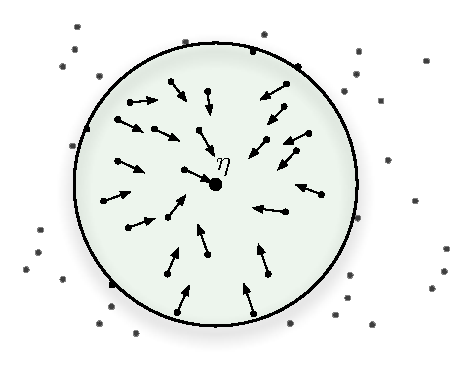
\includegraphics[scale=0.75]{./images02/p1_after_write.pdf}

\caption{Hard-locations pointing, approximately, to the target bitstring.\label{fig-p1-pointers}}
\end{figure}



\subsection{Read operation}

In his work, Kanerva proposed and analyzed a read algorithm called here Kanerva's read. His read takes all activated hard locations counters and sum them. The resulting bitstring has bit $1$ where the result is positive, bit $0$ where the result is negative, and a random bit where the result is zero. In a word, each bit is chosen according to all written bitstrings in all hard locations, being equal to the bit more appeared. Table \ref{tab:kanerva-read} shows an example of Kanerva's read result bitstring.


In this other paragraph we explain what the equator distance is.

Then, this introductory section breaks and moves on to the main findings
of this paper.

% !TEX root = ../partial-sdm.tex

\section{A deviation from the equator distance?}

Kanerva writes\footnote{Email thread `SDM: A puzzling issue and an invitation', started March 16th 2018, in which we discussed the aforementioned discrepancy.  To think that some centuries ago, all scientific publishing was the exchange of such letters.}:

\begin{quote}
    You have done an incredibly thorough analysis of SDM. I like the puzzle in your message and believe that your simulations are correct and to be learned from.  So what to make of the difference compared to my Figure 7.3 (and your Figure \ref{fig:kanerva-figure-73-calculated})?  I think the difference comes from my not having accounted fully for the effect of the other 9,999 vectors that are stored in the memory.  You say in it\\

   ``Our results show that the theoretical prediction is not accurate. There are interaction effects from one or more of the attractors created by the 10,000 writes, and these attractors seem to raise the distance beyond 500 bits (Figure \ref{fig:sdm-10000w-table-7-2}).'' \\

   I think that is correct.  It also brings to mind a comment Louis Jaeckel made when we worked at NASA Ames.  He pointed out that autoassociative storage (each vector is stored with itself as the address) introduces autocorrelation that my formula for Figure 7.2 did not take into account.  When we read from memory, each stored vector exerts a pull toward itself, which also means that each bit of a retrieved vector is slightly biased toward the same bit of the read address, regardless of the read address.  We never worked out the math.
\end{quote}

This is an important observation. A hard location is activated because it shares many dimensions with the items read from or written onto it. Imagine the `counter's eye view':  each individual counter `likes'\footnote{If you are a cell I then I have some serious piece of advice to you.  I would strongly suggest avoiding the neighborhood of a neuron. Neurons have serious authoritarian tendencies, bossing around --- generally electrifying --- the hopeless innocent cells around them just because.} to write on its own corresponding bit-address value more than it likes the opposite; as each hard-location has a say in its own area --- and nowhere else.

Let $x$ and $y$ be random bitstrings and $n$ be the number of dimensions in the memory; let $x_i$ and $y_i$ be the $i$-th bit of $x$ and $y$, respectively; and $d(x, y)$ be the Hamming distance. Whilst the probability of a shared bit-value between same dimension-bits in two random addresses is $1/2$, an address only activates hard-locations close to it.  Let us call these shared bitvalues a \emph{bitmatch in dimension $i$}.

So, what is the probability of bitmatches given that we know the access radius $r$ between the address and a hard-location?
\bigskip

\begin{theorem}
\emph{Each dimension has a small pull bias, which can be measured by}
\label{T1}
$P(x_i = y_i | d(x, y) \le r) = \dfrac{\sum_{k=0}^{r} \binom{n-1}{k}}{\sum_{k=0}^{r} \binom{n}{k}}.$
\end{theorem}

\begin{proof}
    The left-hand expression $P(x_i = y_i | d(x, y) \le r)$ computes the probability of a bitmatch in $i$, given that we know that $x$ and $y$ are in the access radius defined by $r$, i.e., $d(x, y)\le r$.

    Applying the law of total probability to the left-hand expression we obtain

    \begin{align}
    \sum_{k=0}^{r} P(x_i = y_i | d(x, y) = k \le r) P(d(x, y) = k | d(x, y) \le r)
    \end{align}

    We also know that

    \begin{align}
    P(x_i = y_i | d(x, y) = k) &= \frac{n-k}{n} \\
    P(d(x, y) = k | d(x, y) \le r) &= \frac{\binom{n}{k}}{\sum_{j=0}^{r} \binom{n}{j}}
    \end{align}

    Hence,

    \begin{align}
    P(x_i = y_i | d(x, y) \le r) = \frac{\sum_{k=0}^{r} \frac{n-k}{n} \binom{n}{k}}{\sum_{j=0}^{r} \binom{n}{j}}
    \end{align}

    Finally, the combinatorial identity

    \begin{align}
    \frac{n-k}{n} \binom{n}{k} = \frac{(n-k)}{n} \frac{n!}{(n-k)! k!} = \frac{(n-1)!}{k! (n-1-k)!} = \binom{n-1}{k}
    \end{align}

    closes the theorem.

\end{proof}

Theorem \ref{T1} is valid for both ``x written at x'' (autoassociative memory) and ``random written at x'' (heteroassociative memory). When $n=1,000$ and $r=451$, $P(x_i = y_i | d(x, y) \le r) = p = 0.552905498137$.  Each bit of a hard location does indeed have a small pull bias.  What is meant by this is that each particular dimension has a small preference toward positive values if its address bit is set to 1, and negative values if set to 0.


\begin{lemma}
Let $r$ be the access radius given that $f$ percent of the hard locations are activated. Then, $\lim_{n \rightarrow \infty} r/n = 1/2$.
\label{thm:sdm-access-radius}
\end{lemma}
\begin{proof}

As the bits of the hard locations' addresses are randomly chosen, the distance between two hard locations follow a Binomial distribution with $n$ samples and probability 0.5 ($B(n, 0.5)$). For $n$ sufficiently large, the Binomial distribution can be approximated by a Normal distribution, i.e., $B(n, 0.5) \rightarrow \mathcal{N}(\mu = n/2, \sigma^2 = n/4)$.

Let $\Phi(x)$ be the cdf of the standard normal distribution. Let $z = \frac{r - n/2}{\sqrt{n}/2}$. Thus, $P(d(x, y) \le r) = \Phi(z)$. As $f = P(d(x, y) \le r)$, then, $f = \Phi(z)$.

Calculating the inverse, $z = \Phi^{-1}(f)$. Then,

\begin{align}
z &= \Phi^{-1}(f) \\
\frac{r - n/2}{\sqrt{n}/2} &= \Phi^{-1}(f) \\
r &= \frac{n}{2} + \Phi^{-1}(f) \frac{\sqrt{n}}{2} \\
\frac{r}{n} &= \frac{1}{2} + \Phi^{-1}(f) \frac{1}{2 \sqrt{n}}
\end{align}

Therefore, $n \rightarrow \infty \Rightarrow r/n \rightarrow 1/2$.
\end{proof}

\begin{lemma}
Let $\Phi(x)$ be the cdf of the standard normal distribution. Then, $n \rightarrow \infty \Rightarrow P(x_i = y_i | d(x, y) \le r) = \frac{1}{2} \frac{\Phi(z_1)}{\Phi(z_2)}$, where $z_1 = \frac{2r - n + 1}{\sqrt{n-1}}$ and $z_2 = \frac{2r - n}{\sqrt{n}}$.
\label{thm:sdm-T1-n-large}
\end{lemma}
\begin{proof}

From the approximation of the Binomial distribution $B(a, 0.5)$ by the Normal distribution $\mathcal{N}(\mu = a/2, \sigma^2 = a/4)$, we conclude that, for $a$ sufficiently large, the cdf of the Binomial is approximately equal to the cdf of the Normal distribution. Thus,

$$
\frac{1}{2^a} \sum_{k=0}^{b} \binom{a}{k} = \Phi \left( \frac{b-a/2}{\sqrt{a}/2} \right) = \Phi \left( \frac{2b-a}{\sqrt{a}} \right)
$$

Thus,

$$
\sum_{k=0}^{b} \binom{a}{k} = 2^a \Phi \left( \frac{2b-a}{\sqrt{a}} \right)
$$

The result comes directly from applyting the equation above in $P(x_i = y_i | d(x, y) \le r)$.

\end{proof}

\begin{theorem}
The autocorrelation vanishes when $n \rightarrow \infty$, i.e., $\lim_{n \rightarrow \infty} P(x_i = y_i | d(x, y) \le r) = 1/2$.
\label{thm:sdm-autocorrelation-convergence}
\end{theorem}
\begin{proof}

From Lemma \ref{thm:sdm-access-radius}, we know that $r = n/2$ for $n$ sufficiently large. Thus, replacing $r = n/2$ in Lemma \ref{thm:sdm-T1-n-large}, $P(x_i = y_i | d(x, y) \le r) = \frac{\Phi(z_1)}{2 \Phi(z_2)}$, where $z_1 = \frac{1}{\sqrt{n-1}}$ and $z_2 = 0$.

As $n \rightarrow \infty$, $z_1 \rightarrow 0$, and $P(x_i = y_i | d(x, y) \le r) = \frac{\Phi(0)}{2 \Phi(0)} = 1/2$. \qed

Another way to proof is to divide into two cases:

Suppose that $n$ is an even integer, then,

$$
\sum_{k=0}^{r} \binom{n}{k} = \sum_{k=0}^{n/2} \binom{n}{k} = \frac{1}{2} \sum_{k=0}^{n} \binom{n}{k} = \frac{2^n}{2} = 2^{n-1}
$$

And, also,

\begin{align*}
\sum_{k=0}^{r} \binom{n-1}{k} &= \sum_{k=0}^{n/2} \binom{n-1}{k} \\
    &= \frac{1}{2} \left[ \sum_{k=0}^{n-1} \binom{n-1}{k} - \binom{n-1}{n/2} \right] \\
    &= \frac{1}{2} \left[ 2^{n-1} - \binom{n-1}{n/2} \right] \\
    &= 2^{n-2} - \frac{1}{2} \binom{n-1}{n/2}
\end{align*}

Finally,

\begin{align}
P(x_i = y_i | d(x, y) \le r) &= \frac{\sum_{k=0}^{r} \binom{n-1}{k}}{\sum_{k=0}^{r} \binom{n}{k}} \\
    &= \frac{2^{n-2} - \frac{1}{2} \binom{n-1}{n/2}}{2^{n-1}} \\
    &= \frac{2^{n-2}}{2^{n-1}} - \frac{1}{2^n} \binom{n-1}{n/2} \\
    &= \frac{1}{2} - \frac{1}{2^n} \binom{n-1}{n/2}
\end{align}

As $n \rightarrow \infty \Rightarrow \frac{1}{2^n} \binom{n-1}{n/2} \rightarrow 0$, the proof is done for $n$ even.

When $n$ is an odd integer, the steps of the proof are similar. Therefore, the proof is complete.

\end{proof}

In Figure \ref{fig:sdm-10kbits-figure-7-3}, with $n=10,000$ and $r=4,845$, we can notice that the autocorrelation has reduced significantly as predicted by Theorem \ref{thm:sdm-autocorrelation-convergence}. In fact, in this case, using Lemma \ref{thm:sdm-T1-n-large}, $P(x_i = y_i | d(x, y) \le r) = 0.5168761116022098$.

\begin{figure}[!htb]
  \centering
  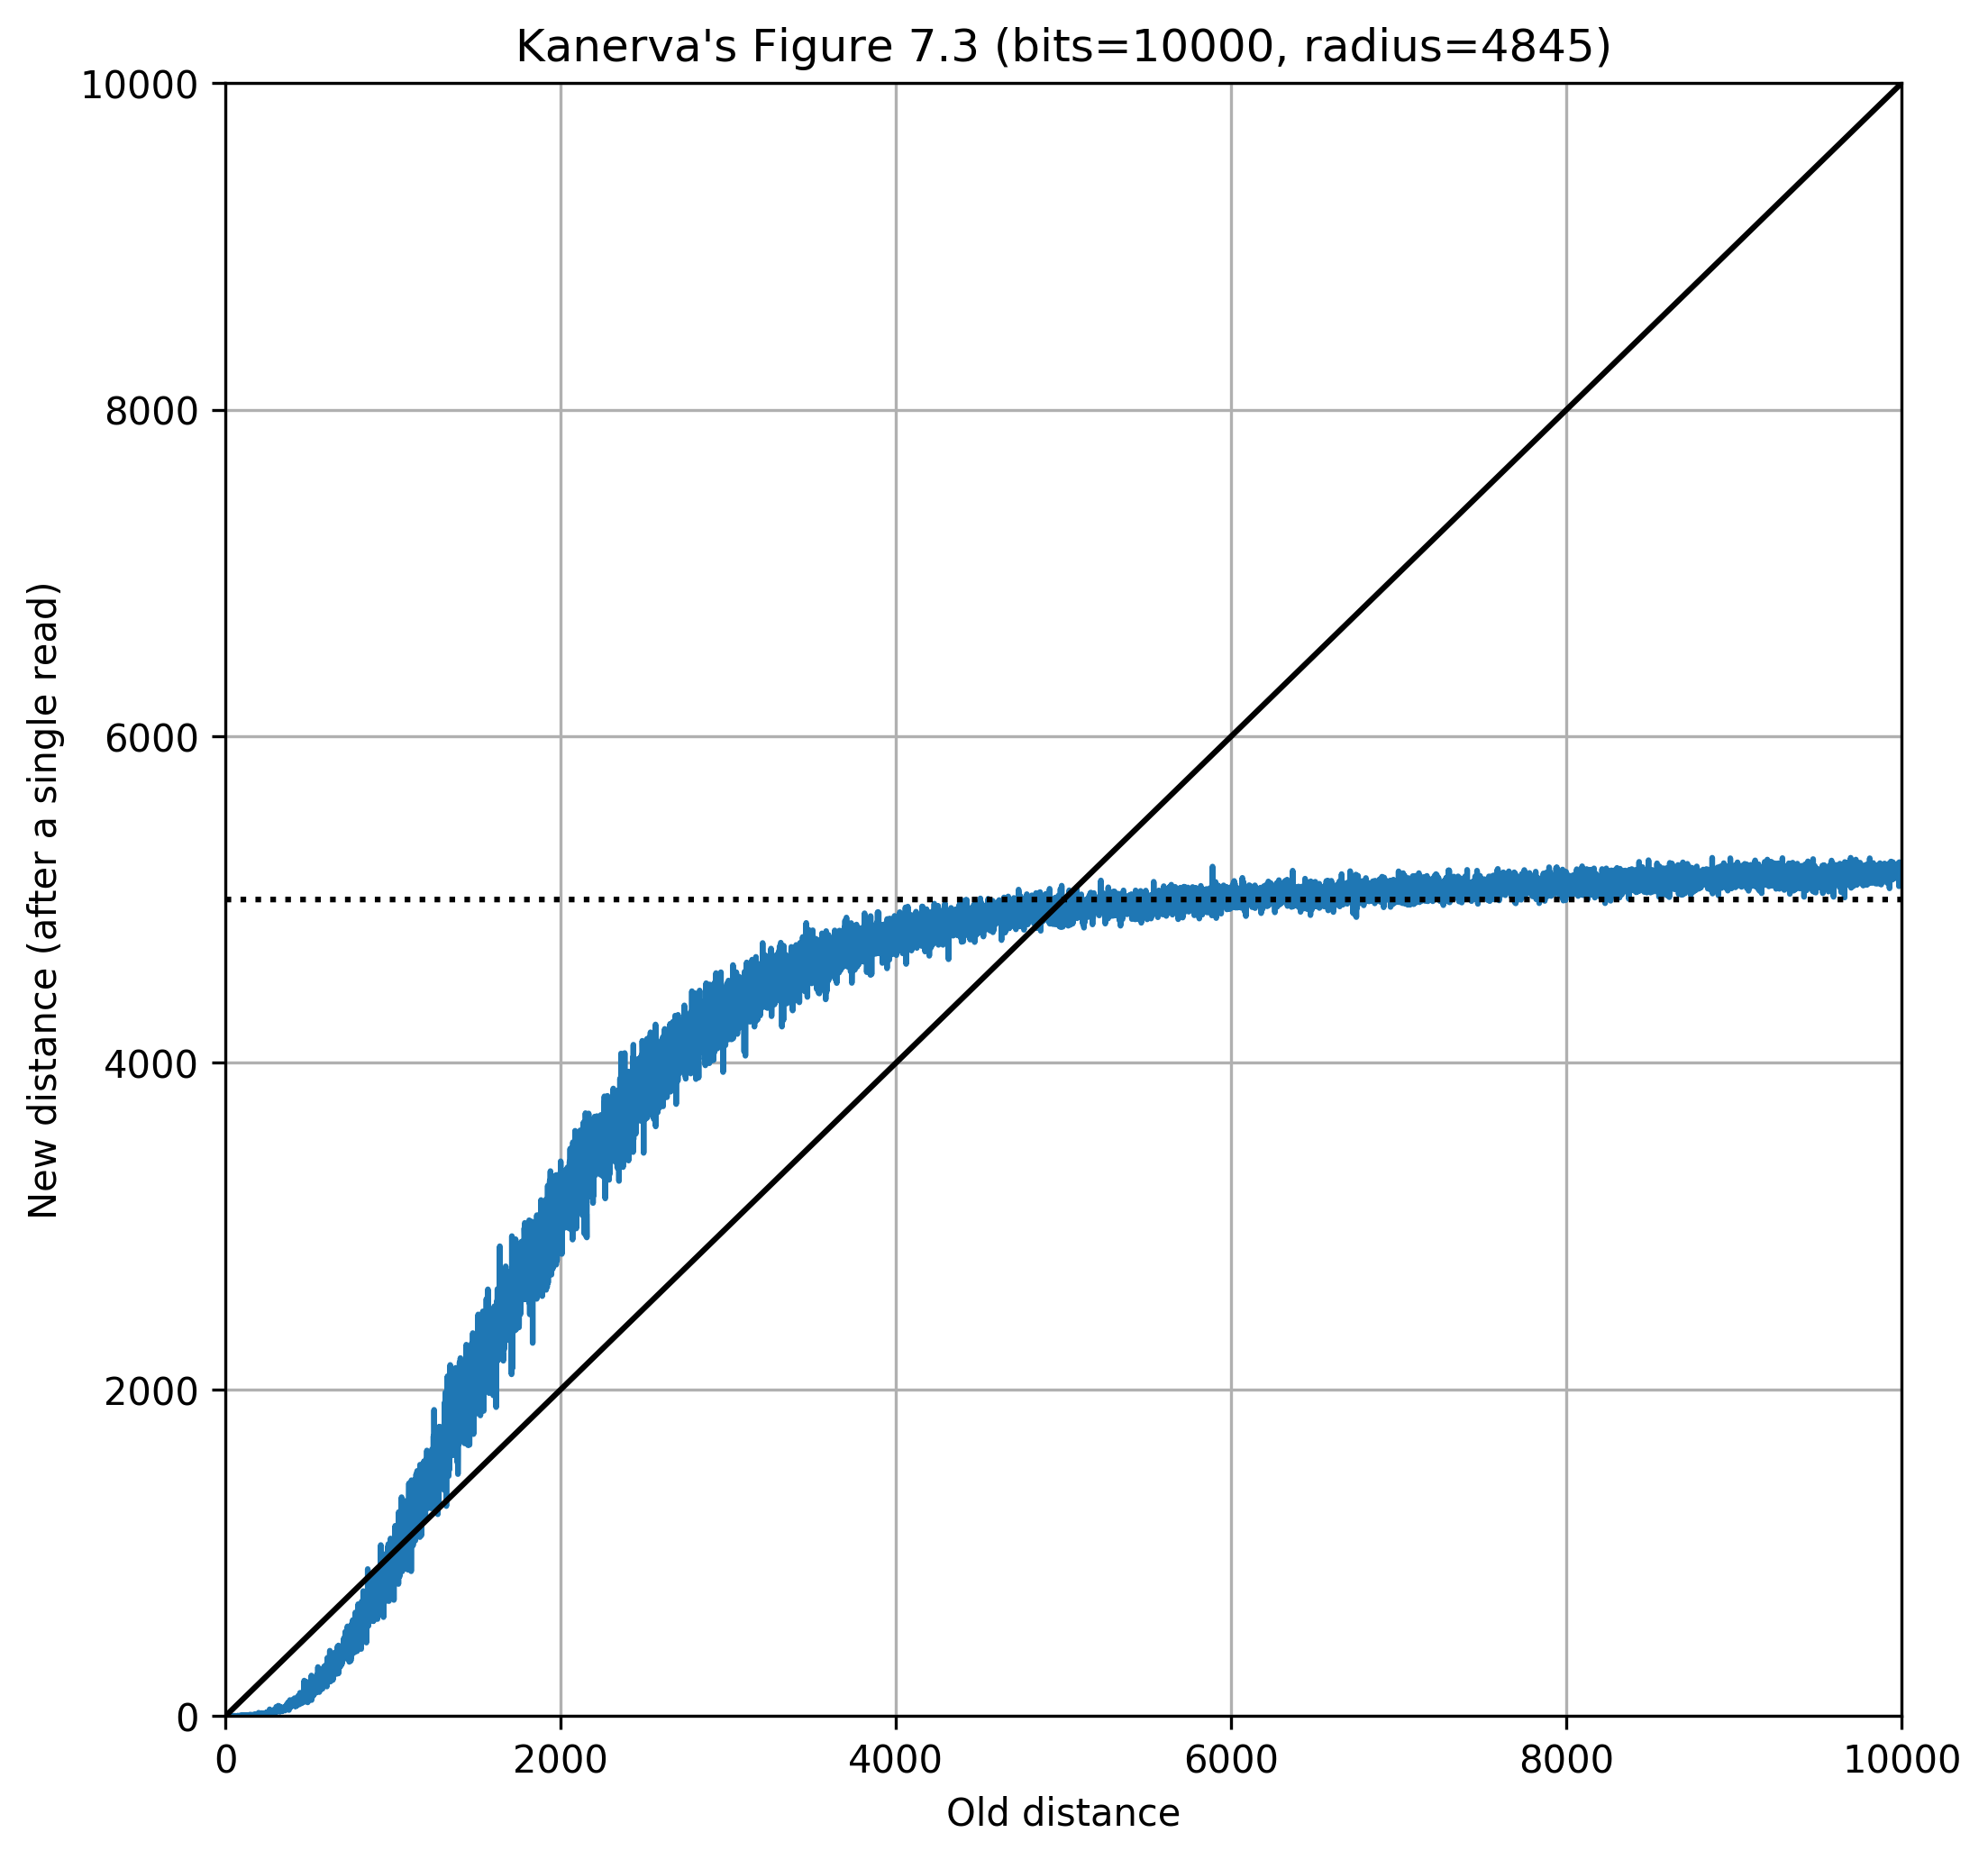
\includegraphics[width=0.75\textwidth]{./images02/sdm-10000bits-10000w-table-7-2.png}

  \caption{The same setup as in Figure \ref{fig:sdm-10000w-table-7-2}, but for $n=10,000$. It shows that the interference has almost gone away when $n$ is sufficiently large.}
  \label{fig:sdm-10kbits-figure-7-3}
\end{figure}

So far we have looked only at a single pair of bitstrings, the probability of a single bitmatch between bitstrings within the access radius distance.  Now let us consider the number of activated hard locations exhibiting this bitmatch.

Let $h$ be the number of activated hard locations. As the probability of activating a specific hard location is constant, $h \sim \text{Binomial}(H, p_1)$. Thus, $\mathbf{E}[h] = \mu_h = Hp_1$ and $\mathbf{V}[h] = \sigma^2_h = Hp_1(1-p_1)$, where $p_1 = 2^{-n} \sum_{k=0}^{r} \binom{n}{k}$.

Let $Z$ be the number of activated hard locations with the same bit as the reading address. Then, $Z = \sum_{i=1}^{h} X_i$, where $X_i \sim \text{Bernoulli}(p)$, where $p = P(x_i = y_i | d(x, y) \le r)$.

\begin{theorem}
Given a reading address $x$ and a dimension $i$, the number of activated hard-locations with bitmatches at $i$ follows a normal distribution with $\mathbf{E}[Z] = \mu_Z = p \mu_h$ and $\mathbf{V}[Z] = \sigma_Z^2 = p(1-p) \mu_h + p^2 \sigma^2_h$.
\label{T2}
\end{theorem}

\begin{proof}
As $P(973 < h < 1170) = 0.997$, by the central limit theorem, $Z$ may be approximated by a normal distribution.

By the central limit theorem, $Z$ is normally distributed.

Applying the law of total averages and the law of total variance, $\mathbf{E}[Z] = \mathbf{E}[\mathbf{E}[Z | h]] = \mathbf{E}[ph] = p \mathbf{E}[h] = ph$, and $\mathbf{V}[Z] = \mathbf{E}[\mathbf{V}[Z|h]] + \mathbf{V}[\mathbf{E}[Z|h]] = \mathbf{E}[hp(1-p)] + \mathbf{V}[ph] = p(1-p) \mathbf{E}[h] + p^2 \mathbf{V}[h] = hp(1-p) + p^2 H p_1 (1-p_1)$.

Applying the law of total variance, $\mathbf{V}[Z] = \mathbf{E}[\mathbf{V}[Z|h]] + \mathbf{V}[\mathbf{E}[Z|h]] = \mathbf{E}[hp(1-p)] + \mathbf{V}[ph] = p(1-p) \mathbf{E}[h] + p^2 \mathbf{V}[h] = p(1-p)\mu_h + p^2 \sigma^2_h$.
\end{proof}


See Figure \ref{fig:sdm-same-bit-histogram} for a comparison between the theoretical model and a simulation.

\begin{figure}[h!]
  \centering
  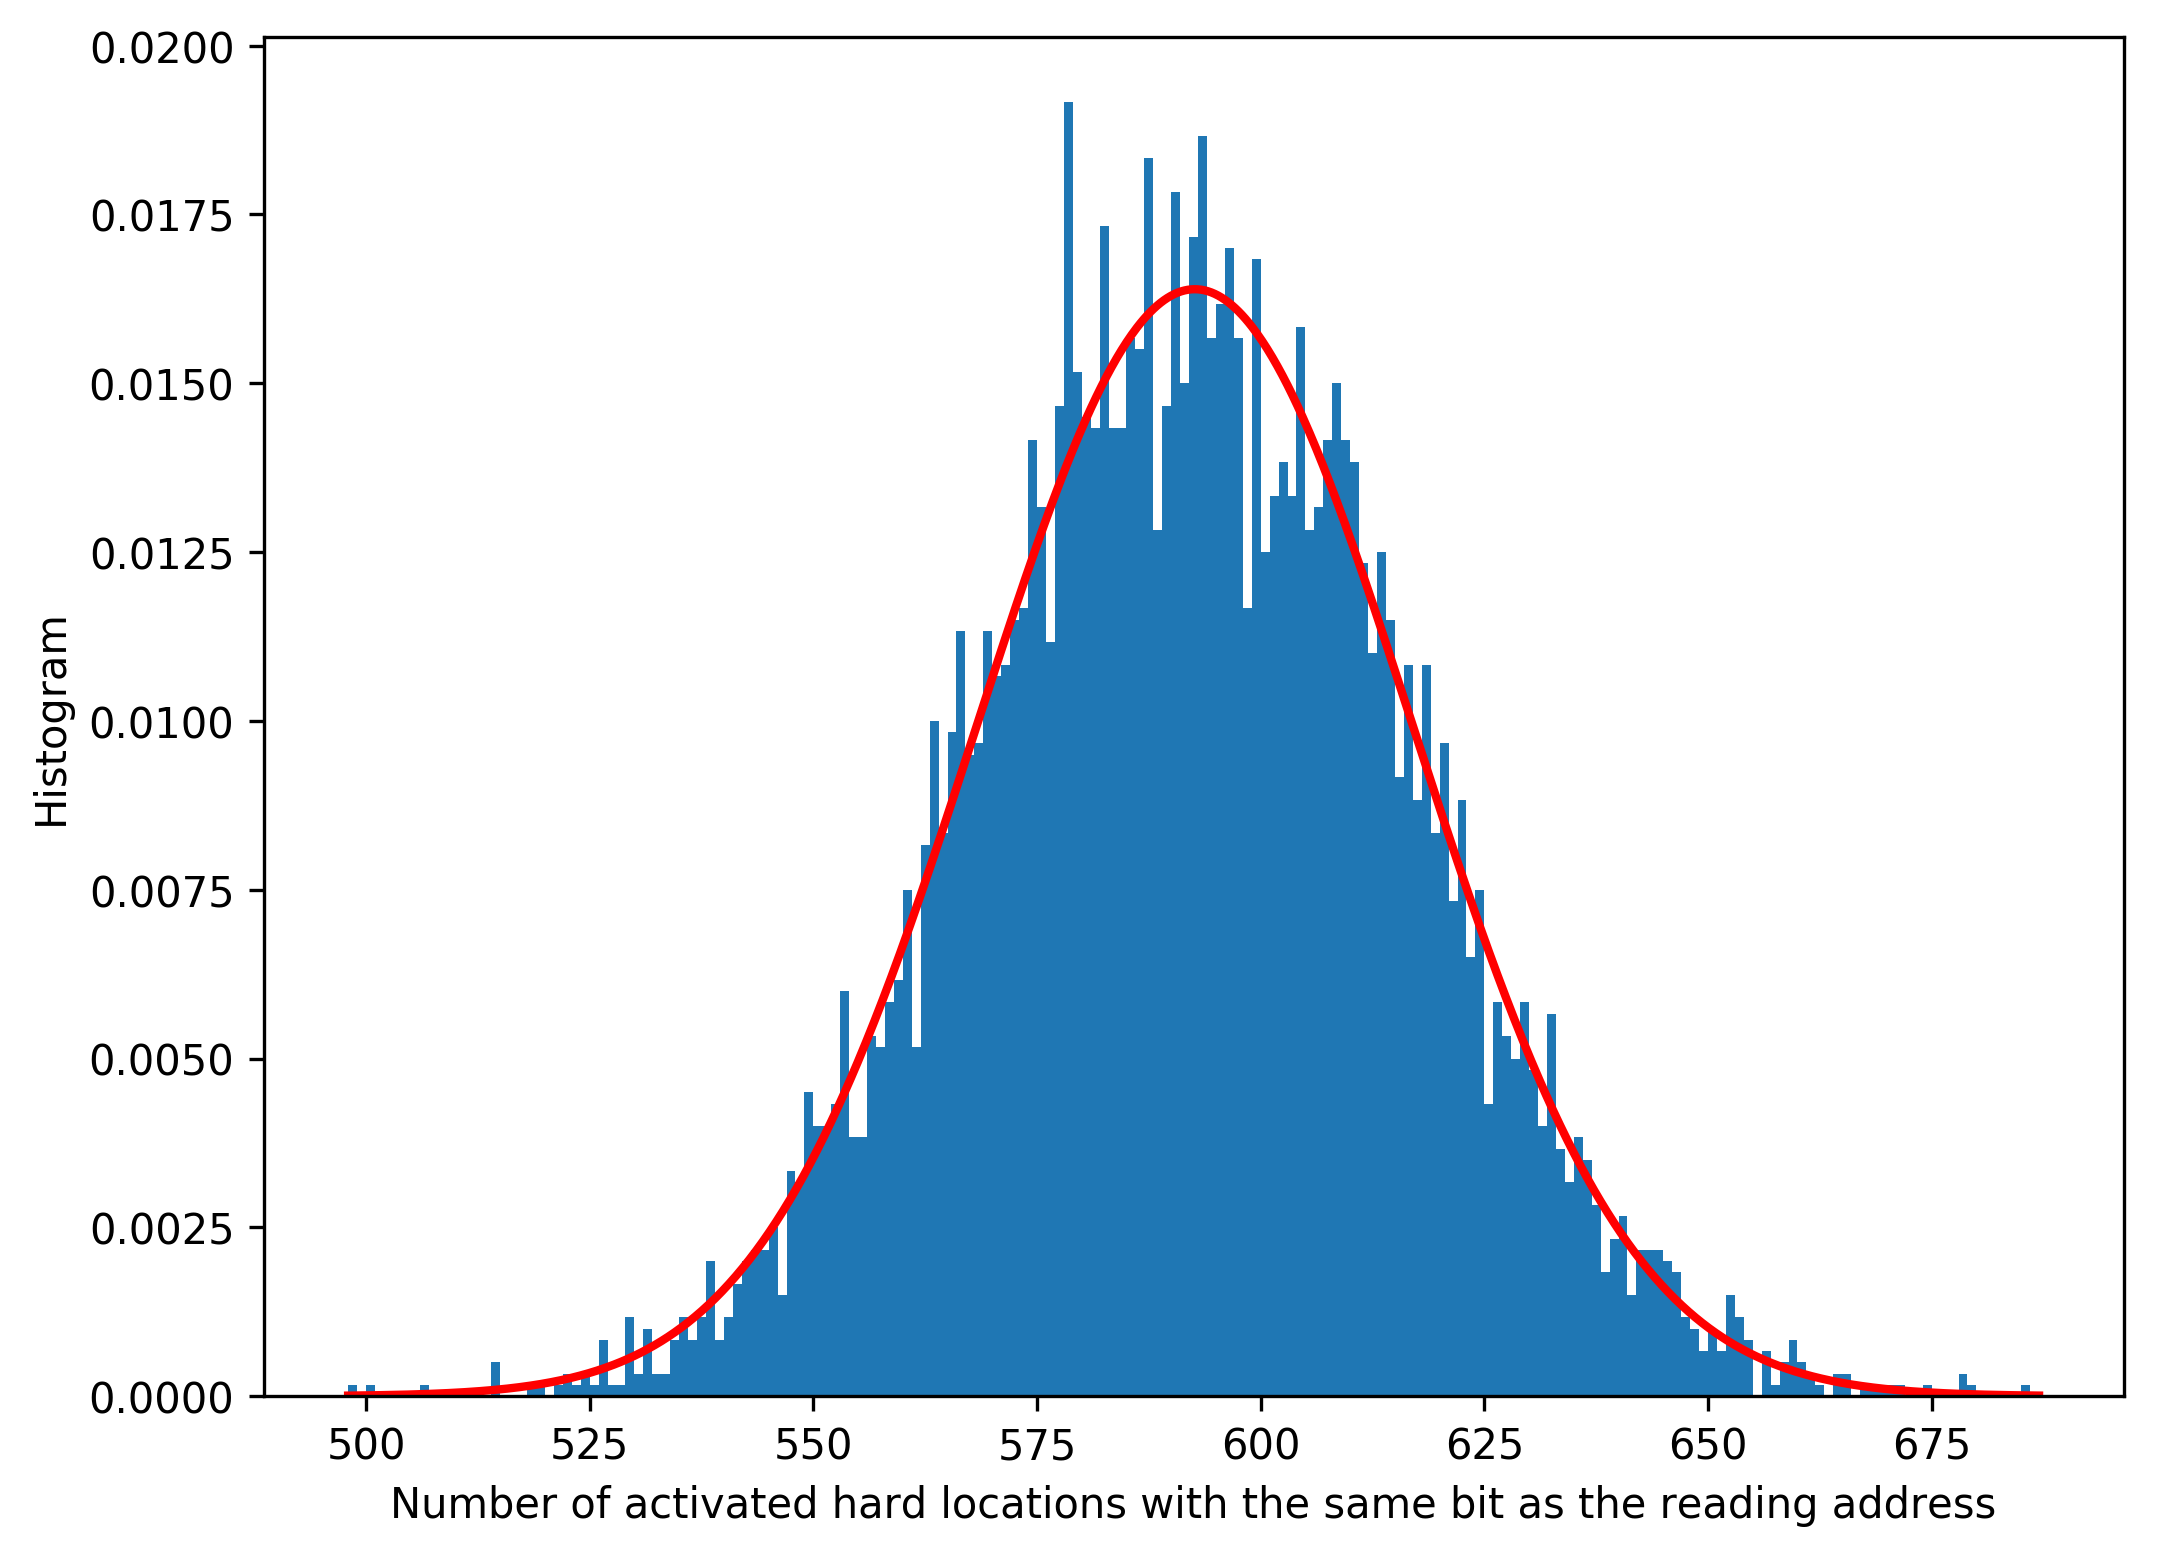
\includegraphics[width=0.75\textwidth]{./images02/autocorrelation/same-bit-histogram.png}

  \caption{Given an address $x$ and a dimension $i$, how many hard locations with bitmatches in $i$ are activated by reading at $x$?  The histogram was obtained through numerical simulation. The red curve is the theoretical normal distribution found in Theorem \ref{T2}.}
  \label{fig:sdm-same-bit-histogram}
\end{figure}

\section{Counter bias}

The previous theorems show that there is bias in the counters. Let us analyze the $i$th counter of a hard location.

Let $s$ be the number of bitstrings written into memory (in our case, $s=10,000$) and $\text{addr}_i$ be the $i$th bit of the hard location's address.

Let $\theta$ be the average number of bitstrings written in each hard location. As there are $s$ bitstrings written into the memory, and the probability of activating a specific hard location is constant, $\theta \sim \text{Binomial}(s, p_1)$. Thus, $\mathbf{E}[\theta] = \mu_\theta = s p_1$ and $\mathbf{V}[\theta] = \sigma^2_\theta = s p_1 (1 - p_1)$.

Let $Y_i$ be the number of bitmatches in the $i$ of a hard location's address after $s$ written bitstrings. Then, $Y_i = \sum_{k=1}^{\theta} X_k$.

\begin{theorem}
Given the number of written bitstrings $s$, $\mathbf{E}[Y_i] = \mu_Y = p \mu_\theta$ and $\mathbf{V}[Y_i] = \sigma^2_Y = p(1-p) \mu_\theta + p^2 \sigma^2_\theta$.
\end{theorem}
\begin{proof}
Applying the law of total expectation, $\mathbf{E}[Y] = \mathbf{E}[\mathbf{E}[Y|\theta]] = \mathbf{E}[p \theta] = p \mathbf{E}[\theta] = p \mu_\theta$.

Applying the law of total variance, $\mathbf{V}[Y] = \mathbf{E}[\mathbf{V}[Y|\theta]] + \mathbf{V}[\mathbf{E}[Y|\theta]] = \mathbf{E}[\theta p (1-p)] + \mathbf{V}[p \theta] = p(1-p) \mathbf{E}[\theta] + p^2 \mathbf{V}[\theta] = p(1-p) \mu_\theta + p^2 \sigma^2_\theta$.
\end{proof}

During a write operation, the counters are incremented for every bit 1 and decremented for every bit 0. So, after $s$ writes, there will be $\theta$ bitstrings written in each hard location with $Y_i$ bitmatches and $\theta - Y_i$ non-bitmatches. Thus, $[\text{cnt}_i | \text{addr}_i = 1] = (Y_i) - (\theta - Y_i) = 2Y_i - \theta$ and $[\text{cnt}_i | \text{addr}_i = 0] = \theta - 2Y_i$.

\begin{theorem}
$\mathbf{E}[\text{cnt}_i | \text{addr}_i = 1] = \mu_{\text{cnt}} = (2p-1) \mu_\theta$ and $\mathbf{V}[\text{cnt}_i | \text{addr}_i = 1] = \sigma^2_\text{cnt} = 4p(1-p) \mu_\theta + (2p-1)^2 \sigma^2_\theta$.
\end{theorem}

\begin{proof}

$\mathbf{E}[\text{cnt}_i | \text{addr}_i = 1] = \mathbf{E}[2Y_i - \theta] = \mathbf{E}[2Y_i] - \mathbf{E}[\theta] = 2 \mathbf{E}[Y_i] - \mu_\theta = 2 p \mu_\theta - \mu_\theta = (2p-1) \mu_\theta$.

Applying the law of total variance, $\mathbf{V}[\text{cnt}_i | \text{addr}_i = 1] = \mathbf{V}[2Y_i - \theta] = \mathbf{E}[\mathbf{V}[2Y_i - \theta | \theta]] + \mathbf{V}[\mathbf{E}[2Y_i - \theta | \theta]]$.

Let us solve each part independently. Thus,

$\mathbf{V}[2Y_i - \theta | \theta] = \mathbf{V}[2Y_i | \theta] = 4 \mathbf{V}[Y_i | \theta] = 4 \mathbf{V}[\sum_{k=1}^\theta X_k] = 4 \theta p (1-p)$.

$\mathbf{E}[\mathbf{V}[2Y_i - \theta | \theta]] = \mathbf{E}[4 \theta p (1-p)] = 4p(1-p) \mathbf{E}[\theta] = 4p(1-p) \mu_\theta$.

Finally,

$\mathbf{E}[2Y_i - \theta | \theta] = 2 \mathbf{E}[Y_i | \theta] - \mathbf{E}[\theta | \theta] = 2p \theta - \theta = (2p-1) \theta$.

$\mathbf{V}[\mathbf{E}[2Y_i - \theta | \theta]] = \mathbf{V}[(2p-1) \theta] = (2p-1)^2 \mathbf{V}[\theta] = (2p-1)^2 \sigma^2_\theta$.
\end{proof}

\begin{theorem}
$\mathbf{E}[\text{cnt}_i | \text{addr}_i = 0] = - \mu_{\text{cnt}}$ and $\mathbf{V}[\text{cnt}_i | \text{addr}_i = 1] = \sigma^2_\text{cnt}$.
\end{theorem}
\begin{proof}
Notice that $[\text{cnt}_i | \text{addr}_i = 0] = -[\text{cnt}_i | \text{addr}_i = 1]$. Thus, $\mathbf{E}[\text{cnt}_i | \text{addr}_i = 0] = -\mathbf{E}[\text{cnt}_i | \text{addr}_i = 1]$ and $\mathbf{V}[\text{cnt}_i | \text{addr}_i = 0] = \mathbf{V}[\text{cnt}_i | \text{addr}_i = 1]$.
\end{proof}

In summary,

\begin{align}
\left[ \text{cnt}_i | \text{addr}_i=1 \right] &\sim \mathcal{N}(\mu_\text{cnt}, \sigma^2_\text{cnt})\label{cntaddr1} \\
\left[ \text{cnt}_i | \text{addr}_i=0 \right] &\sim \mathcal{N}(-\mu_\text{cnt}, \sigma^2_\text{cnt})\label{cntaddr0}
\end{align}

In our case, $p=0.5529$, $s=10,000$, and $H=1,000,000$, so $[\text{cnt}_i | \text{addr}_i=1] \sim \mathcal{N}(\mu=1.1341, \sigma^2 = 10.7184)$. For ``random at x'', $p=0.5$, so $\mu = 0$ and $\sigma^2 = 10.7185$. See Figure \ref{fig:sdm-corr-counters}.

\begin{figure}[h!]
  \centering
  \subfloat[$\text{addr}_i=1$]{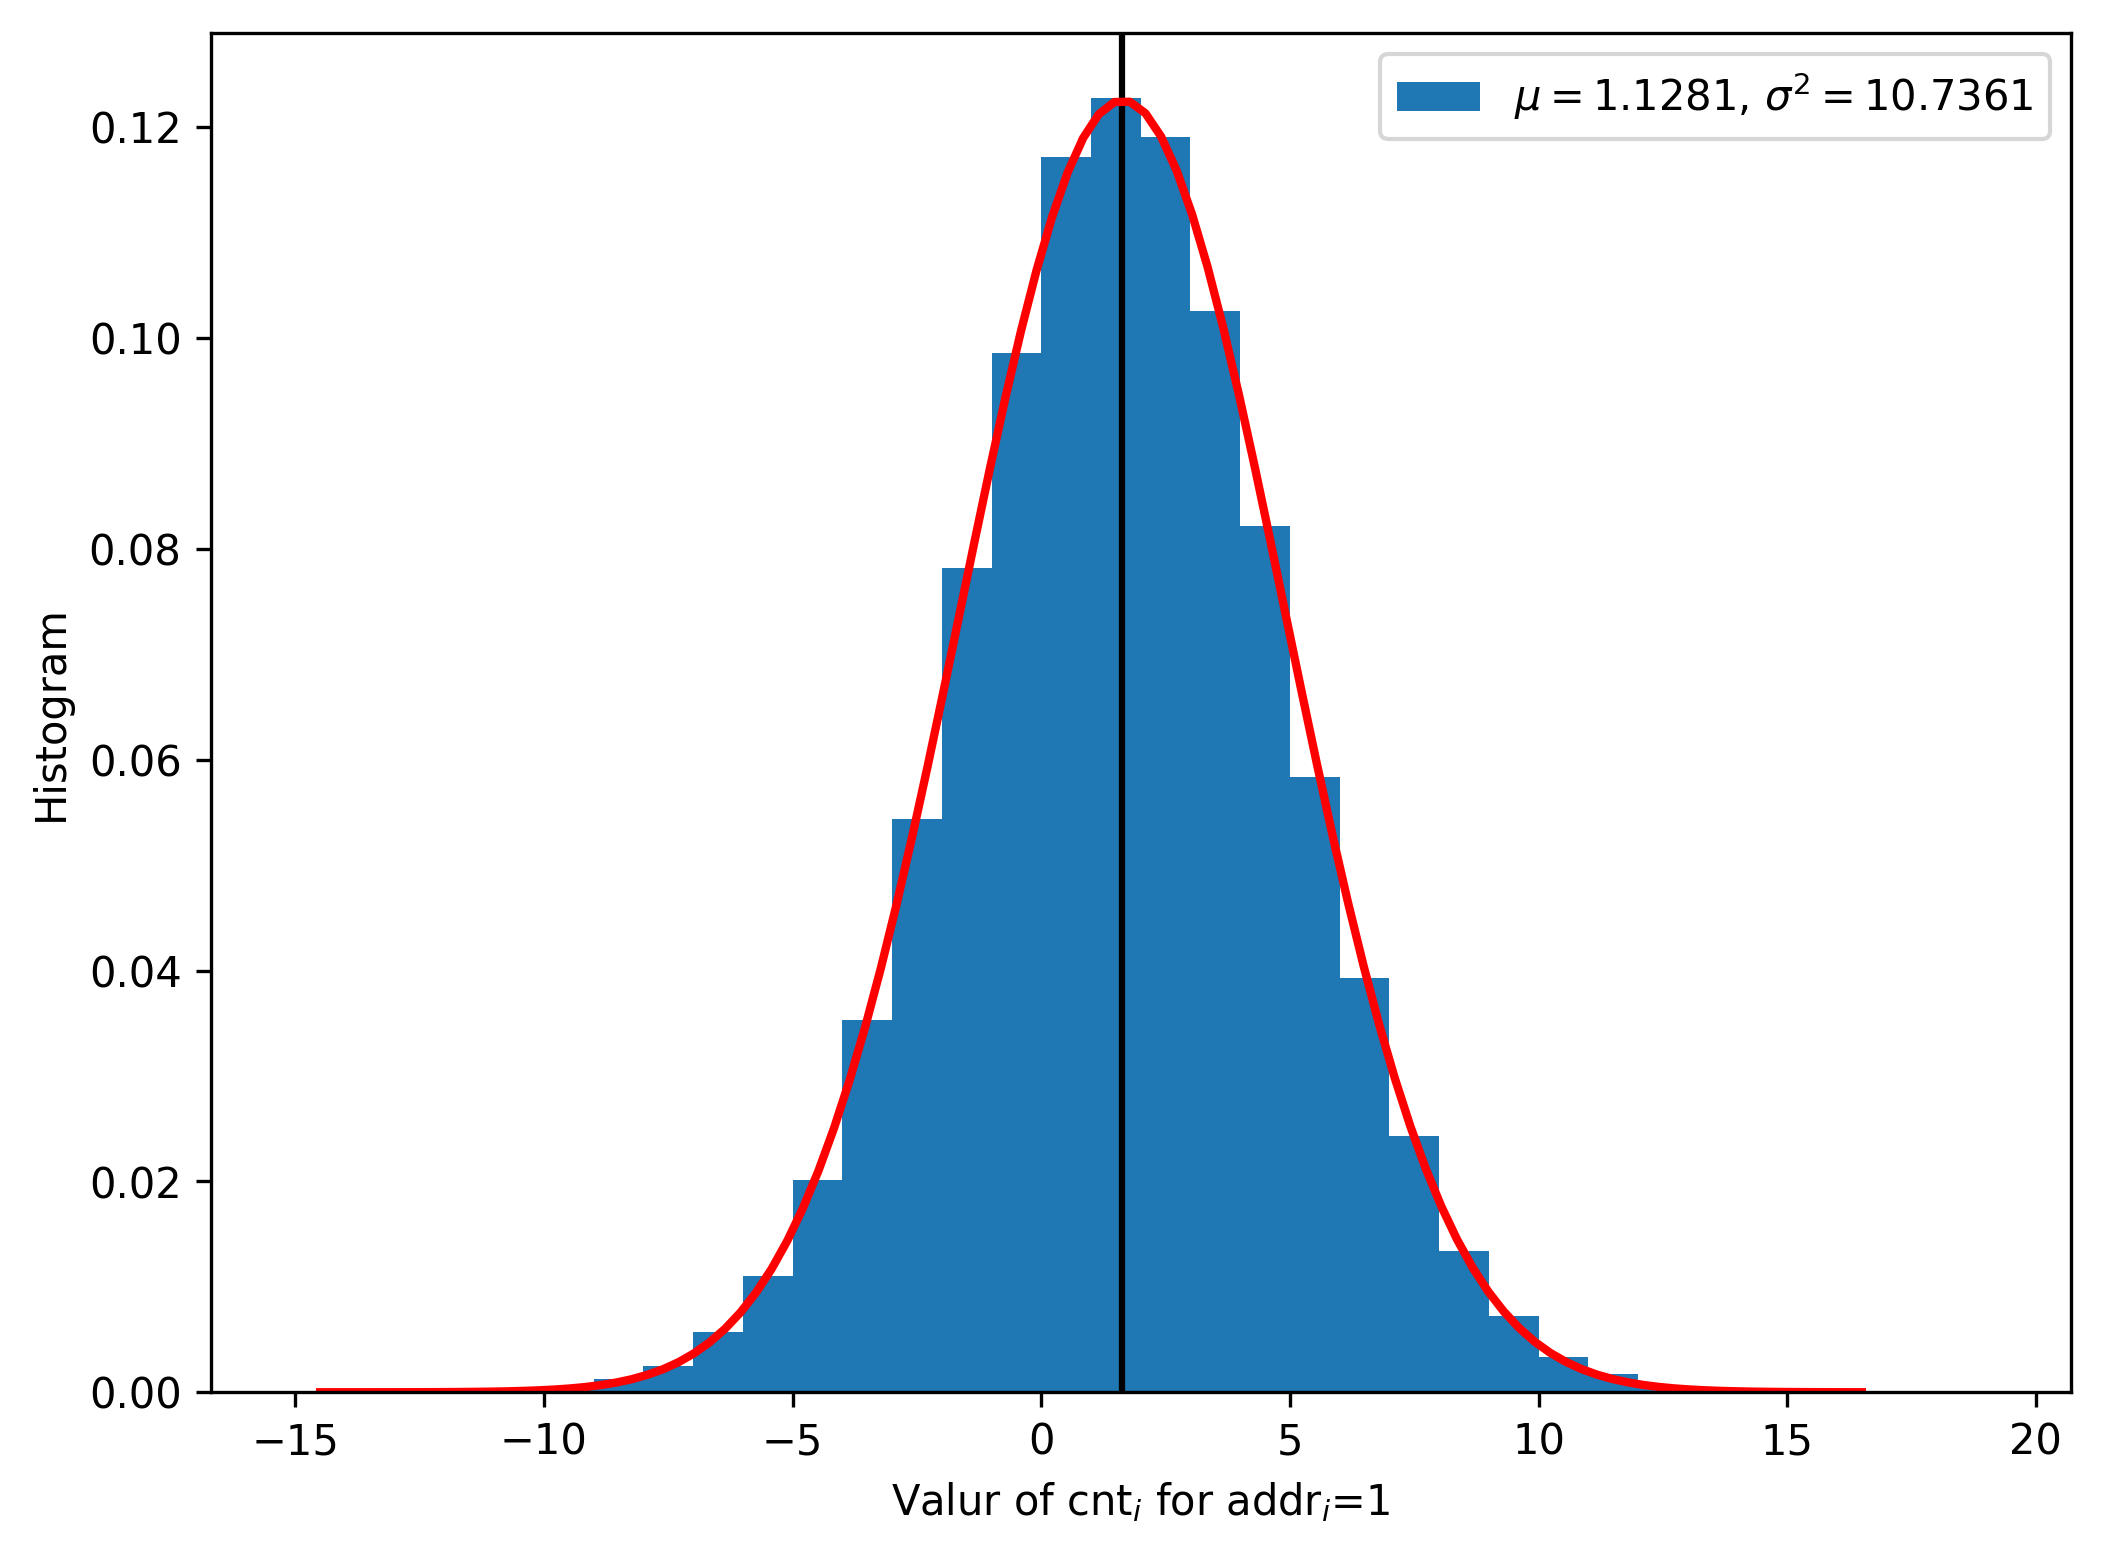
\includegraphics[width=0.5\textwidth]{./images02/autocorrelation/x_at_x_addr1.png}}
  \subfloat[$\text{addr}_i=0$]{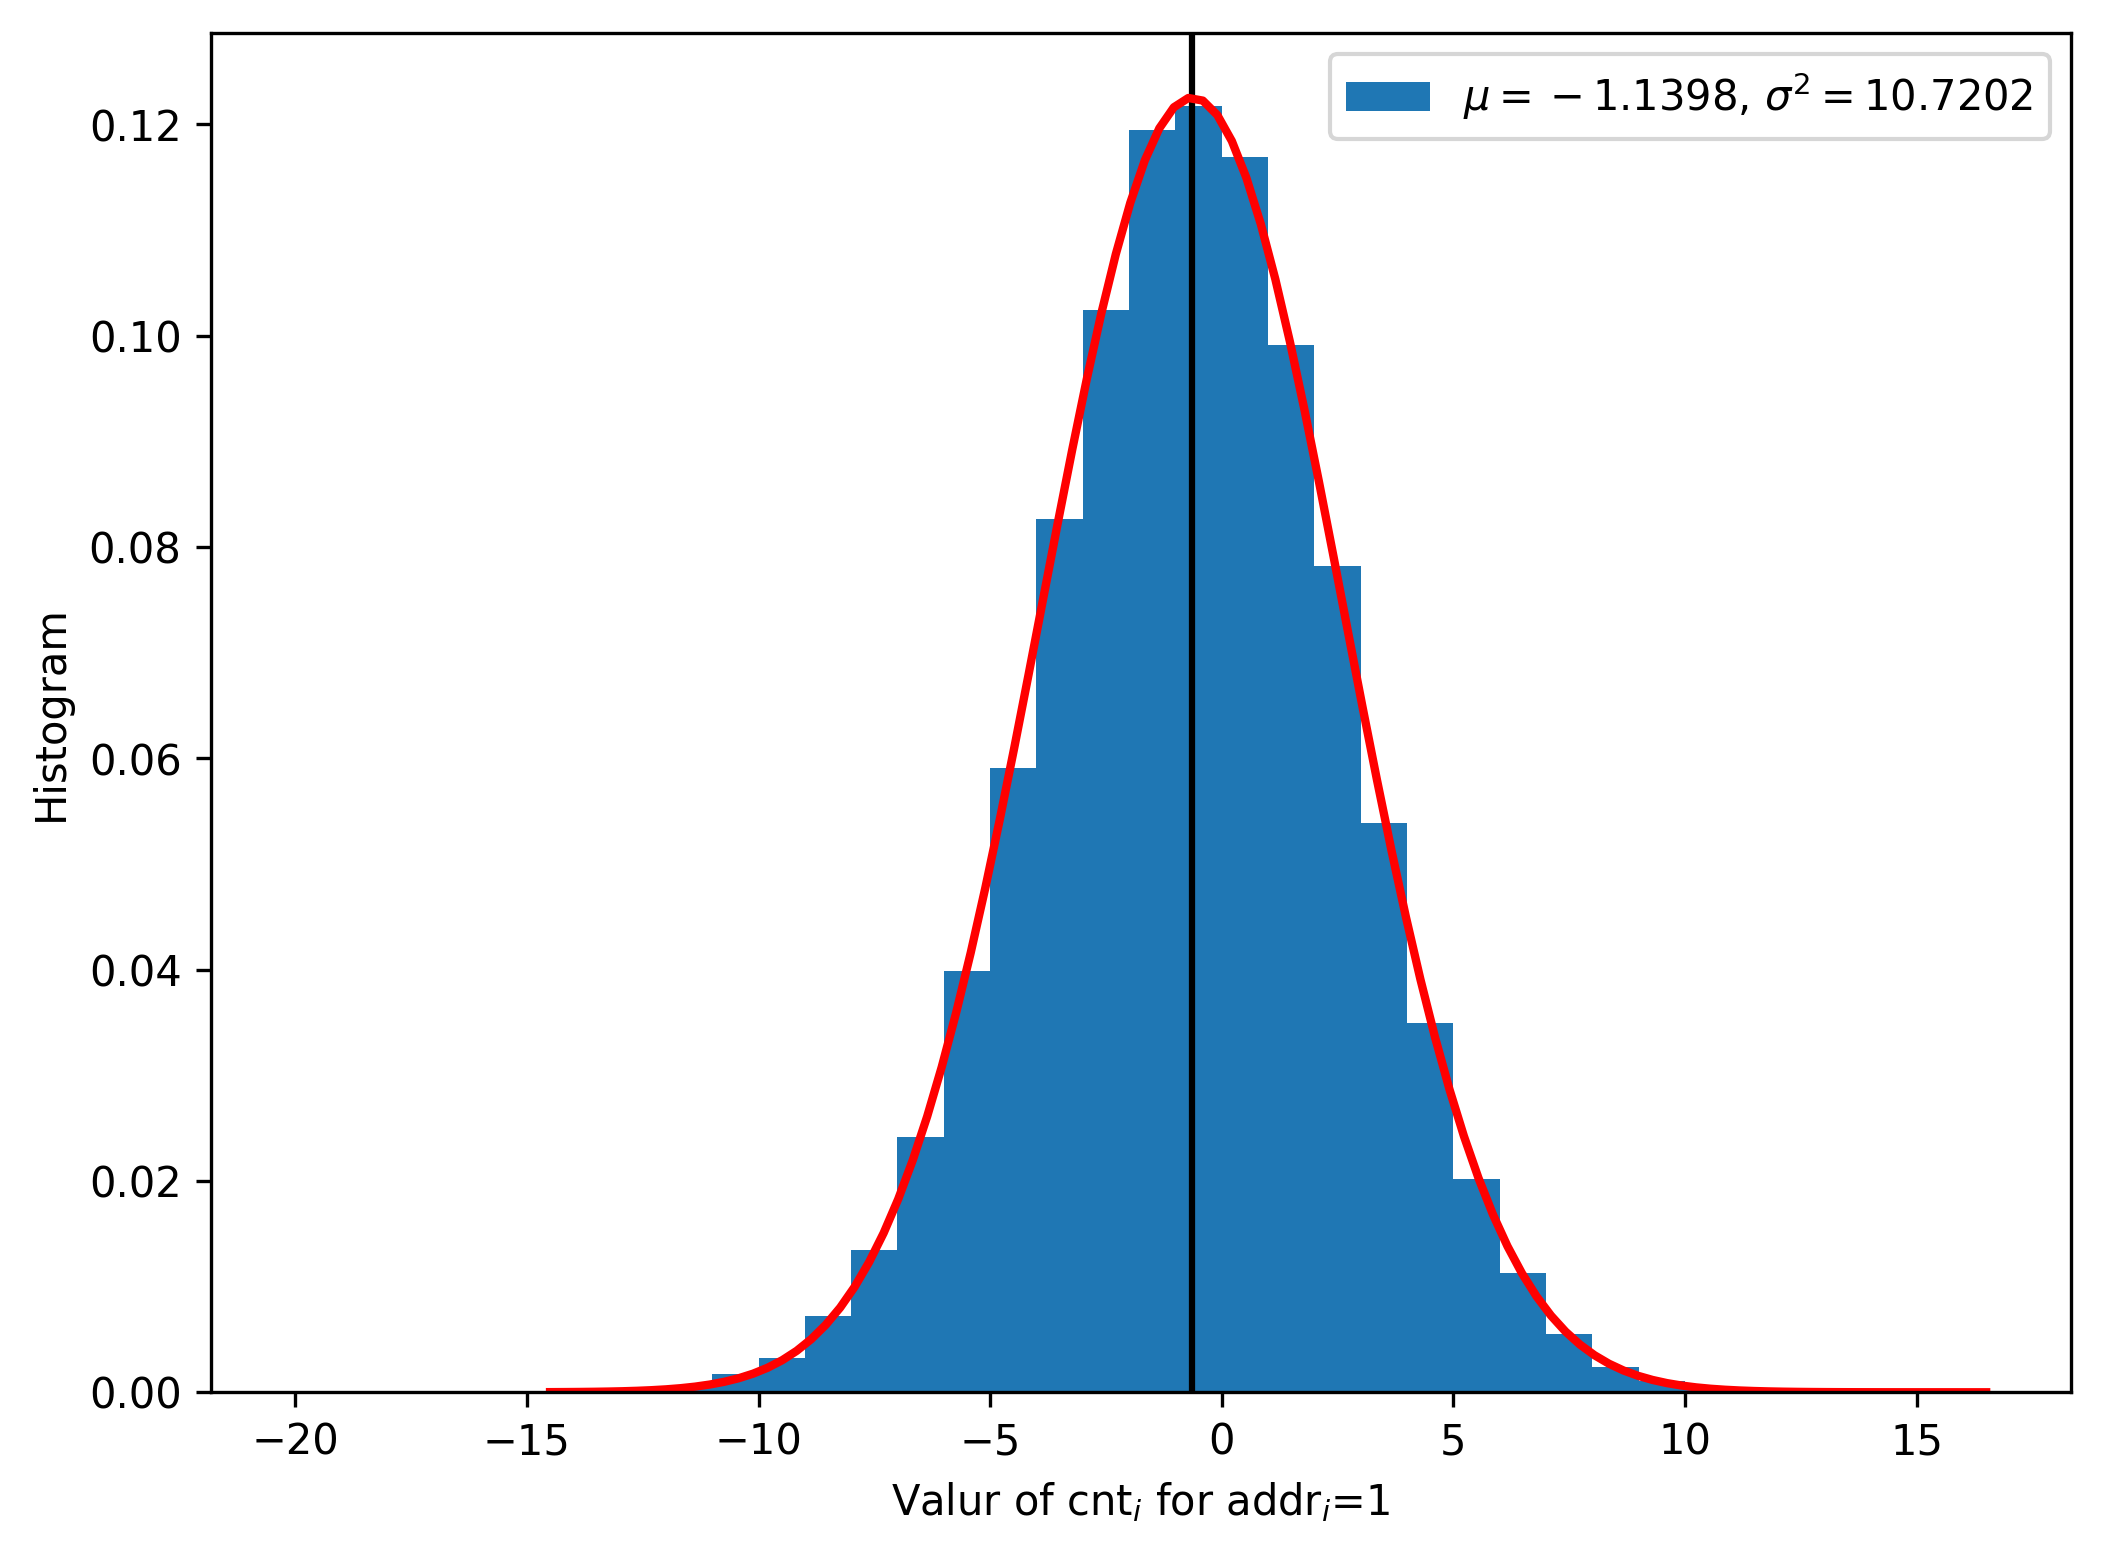
\includegraphics[width=0.5\textwidth]{./images02/autocorrelation/x_at_x_addr0.png}}

  \caption{The value of the counters after $s=10,000$ writes shows the autocorrelation in the counters in autoassociative memories (``x at x''). The histogram was obtained through simulation. The red curve is the theoretical normal distribution found in equations (\ref{cntaddr1}) and (\ref{cntaddr0}).}
  \label{fig:sdm-corr-counters}
\end{figure}


Finally,

\begin{align}
P(\text{cnt}_i > 0 | \text{addr}_i = 1) = P(\text{cnt}_i < 0 | \text{addr}_i = 0) = 1 - \mathcal{N}.\text{cdf}(0)
\end{align}

For ``random written at x'', $p=0.5$ implies $\mu_\text{cnt} = 0$, which implies $P(\text{cnt}_i > 0 | \text{addr}_i = 1) = P(\text{cnt}_i < 0 | \text{addr}_i = 0) = 0.5$, independently of the parameters because they will only affect the variance and the normal distribution is symmetrical around the average.

However, for ``x written at x'', $p=0.5529$ and the probabilities depend on $s$. For $s=10,000$, they are equal to 0.6354. For $s=20,000$, they are equal to 0.6867. For $s=30,000$, they are equal to 0.7232. The more random bitstrings are written into the memory, the more the hard locations point to themselves.

Let $D$ be the number of counters aligned with $\text{addr}_i$. The standard deviation was calculated using the fact that $[D|\theta] \sim \text{Binomial}(1000, q=P(\text{cnt}_i > 0 | \text{addr}_i=1, \theta))$.

Applying the law of total variance, $\mathbf{V}[D] = \mathbf{E}[\mathbf{V}[D|\theta]] + \mathbf{V}[\mathbf{E}[D|\theta]] = \mathbf{E}[1000 q (1-q)] + \mathbf{V}[1000 q] = 1000 \mathbf{E}[q-q^2] + 1000^2 \mathbf{V}[q] = 1000 \mathbf{E}[q](1-\mathbf{E}[q]) + 1000(1000-1)\mathbf{V}[q]$, where $\mathbf{E}[q] = \sum_\theta P(\text{cnt}_i > 0 | \text{addr}_i=1, \theta) P(\theta)$ and $\mathbf{E}[q^2] = \sum_\theta [P(\text{cnt}_i > 0 | \text{addr}_i=1, \theta)]^2 P(\theta)$.

Doing the math, $\mathbf{E}[q] = 0.402922$ and $\mathbf{E}[q^2] = 0.634433$. Thus, $\mathbf{V}[q] = \mathbf{E}[q^2] - (\mathbf{E}[q])^2 = 0.0004166$. Hence, $\mathbf{V}[D] = 648.2041$. See Figure \ref{fig:sdm-corr-prob} and notice that I still have to figure out why the mean is correct, but the standard deviation is not.

\begin{figure}[h!]
  \centering
  \subfloat[``random at x'']{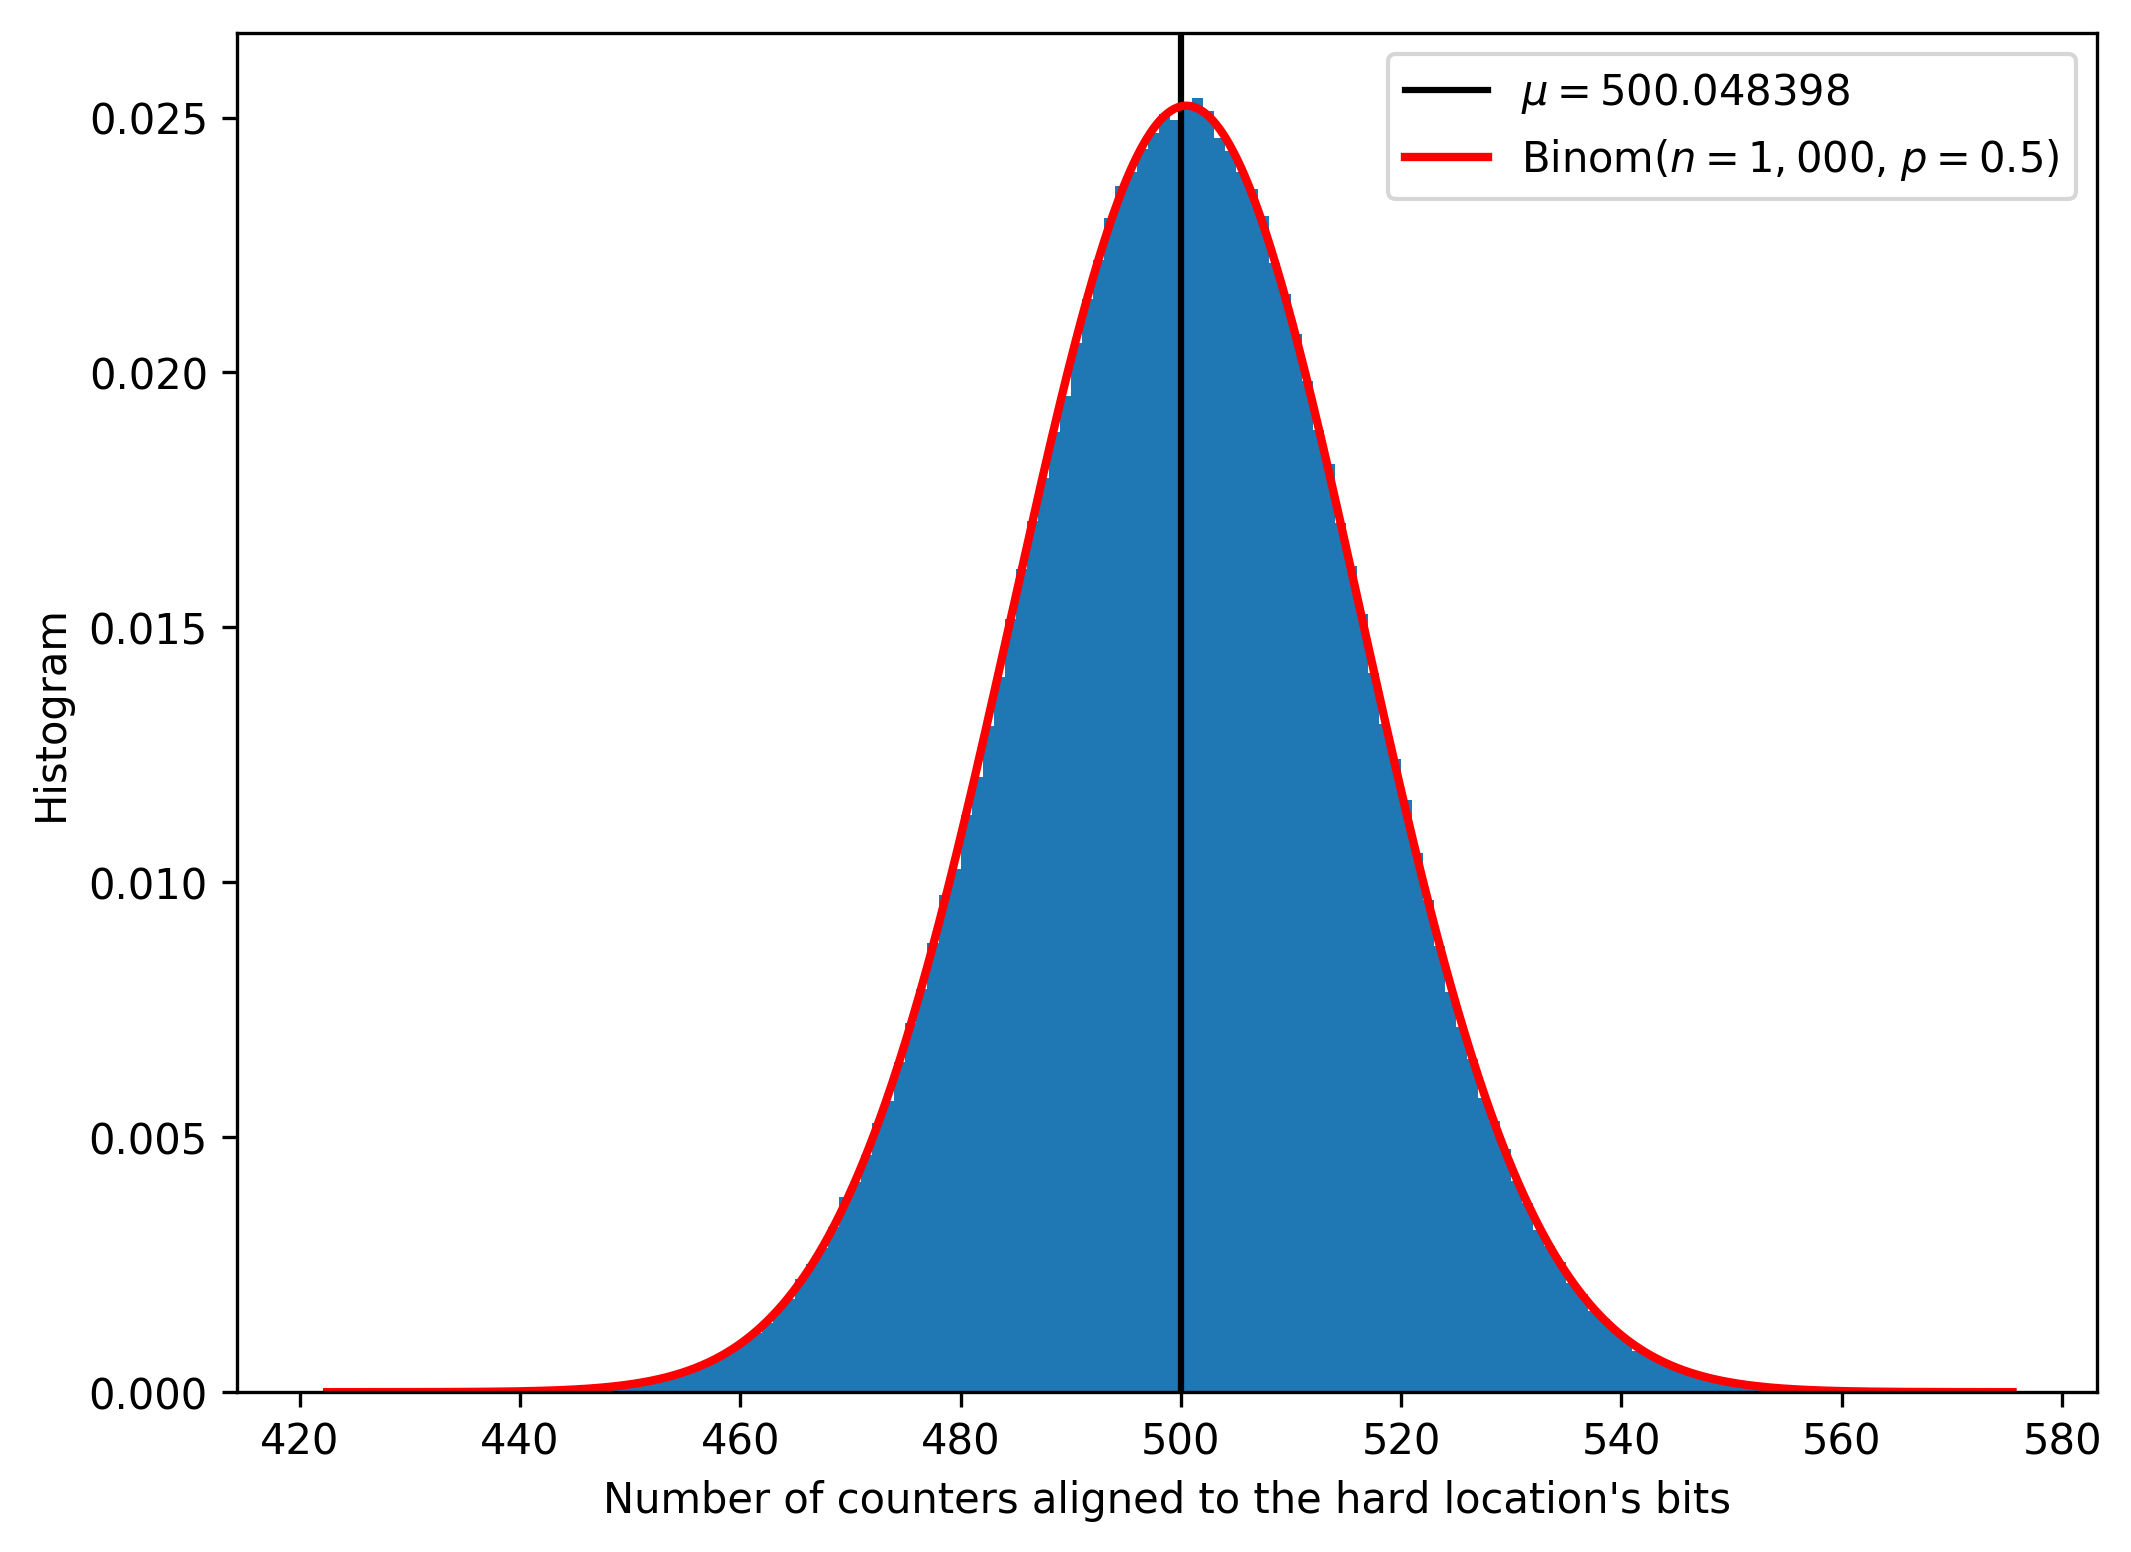
\includegraphics[width=0.5\textwidth]{./images02/autocorrelation/random_at_x_counters.png}}
  \subfloat[``x at x'']{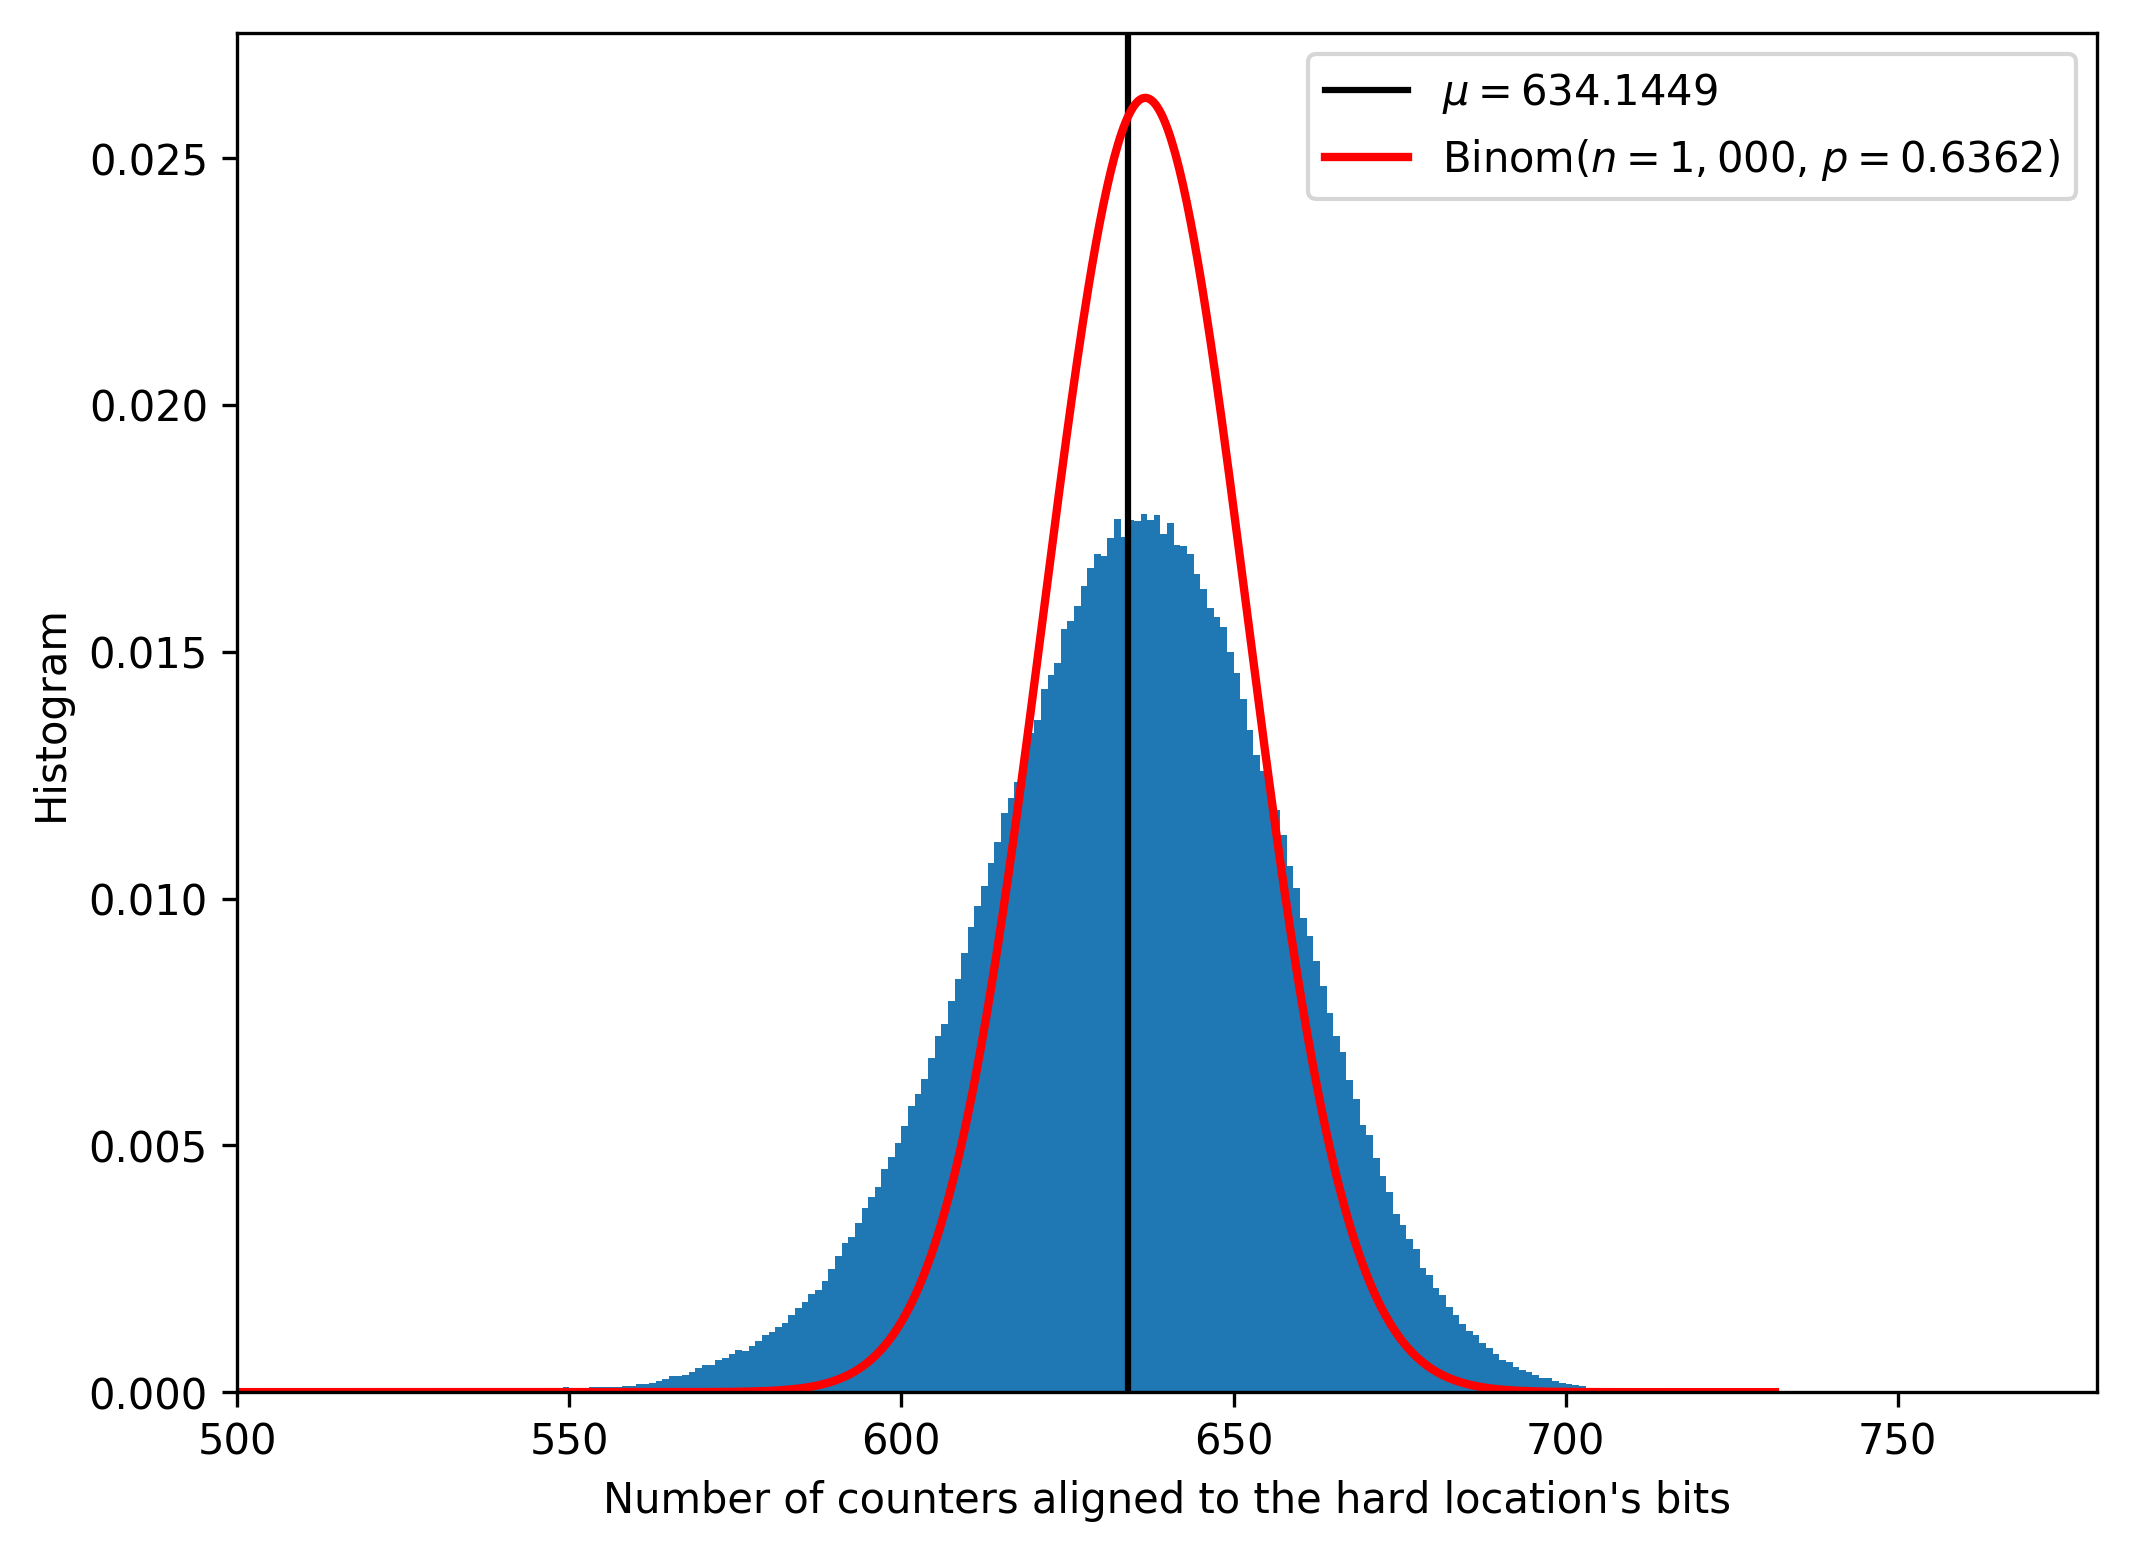
\includegraphics[width=0.5\textwidth]{./images02/autocorrelation/x_at_x_counters.png}}

  \caption{Autocorrelation in the counters in autoassociative memories (``x written at x''). The histogram was obtained through simulation. The red curve is the theoretical distribution.}
  \label{fig:sdm-corr-prob}
\end{figure}



\section{Read bias}

Now that we know the distribution of $\text{cnt}_i | \text{addr}_i$, we may go to the read operation. During the read operation, on average, $h$ hard locations are activated and their counters are summed up. So, for the $i$th bit,

\begin{align}
\text{acc}_i = \sum_{k=1}^{h} \text{cnt}_k
\end{align}

Let $\eta$ be the reading address and $\eta_i$ the $i$th bit of it. Then, let's split the $h$ activated hard locations into two groups: (i) the ones with the same bit as $\eta_i$ with $Z$ hard locations, and (ii) the ones with the opposite bit as $\eta_i$ with $h-Z$ hard locations.

\begin{align}
\left[ \text{acc}_i|\eta_i \right] &= \sum_{k=1}^{Z} \left[ \text{cnt}_k | \text{addr}_k=\eta_i \right] + \sum_{k=1}^{h-Z} \left[ \text{cnt}_k | \text{addr}_k \ne \eta_i \right]
\end{align}

Each sum is a sum of normally distributed random variables, so

\begin{align}
\sum_{k=1}^{Z} \left[ \text{cnt}_k | \text{addr}_k=\eta_1 \right] &\sim \mathcal{N}(\mu = \mu_\text{cnt} \mu_Z, \sigma^2 = \sigma_\text{cnt}^2 \mu_Z + \mu_\text{cnt}^2 \sigma^2_Z) \label{eqn:sdm-eta1-addr1} \\
\sum_{k=1}^{h-Z} \left[ \text{cnt}_k | \text{addr}_k \ne \eta_1 \right] &\sim \mathcal{N}(\mu = -\mu_\text{cnt} (1-p) \mu_h, \sigma^2 = \sigma^2_\text{cnt} (1-p) \mu_h + \mu_\text{cnt}^2 \sigma^2_{h-Z}) \label{eqn:sdm-eta1-addr0}
\end{align}

In our case, $\sum_{k=1}^{Z} \left[ \text{cnt}_k | \text{addr}_k=1 \right] \sim \mathcal{N}(\mu=672.12, \sigma^2=7113.87)$, and $\sum_{k=1}^{Z} \left[ \text{cnt}_k | \text{addr}_k=1 \right] \sim \mathcal{N}(\mu=-543.49, \sigma^2=5752.54)$. See Figure \ref{fig:sdm-read-sums} --- we can notice that the average is correct but the variance is too small.

\begin{figure}[h!]
  \centering
  \subfloat[Equation \ref{eqn:sdm-eta1-addr1}  ($\text{addr}_k=1)$]{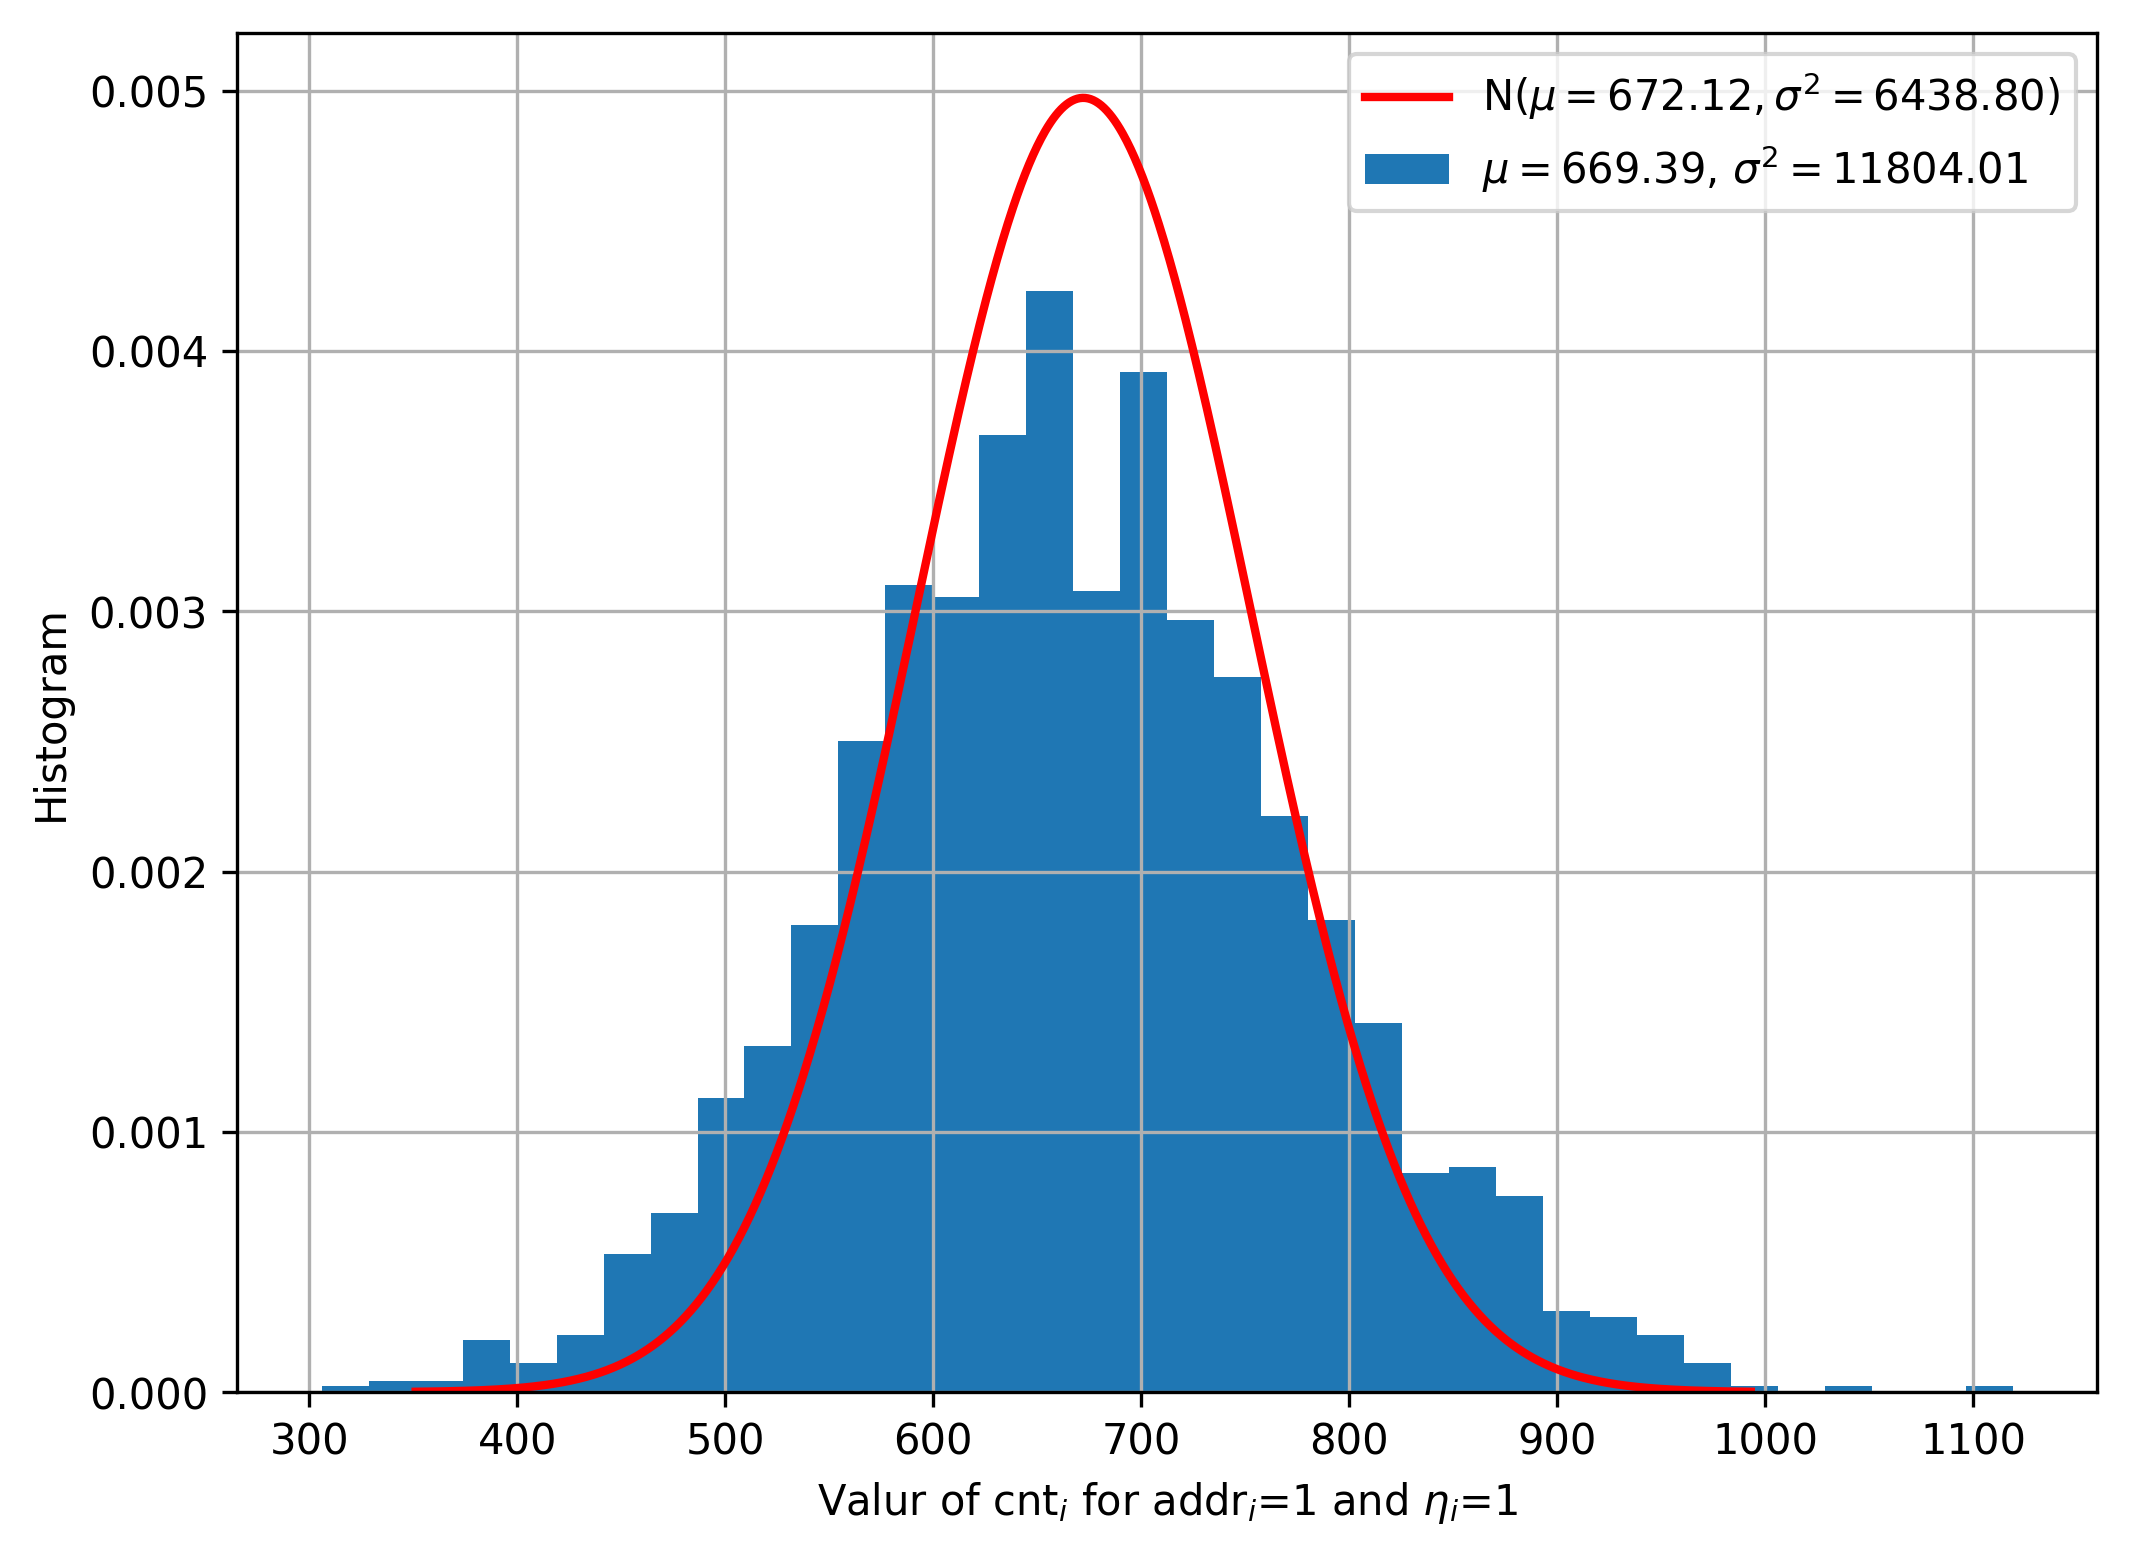
\includegraphics[width=0.5\textwidth]{./images02/autocorrelation/read-counters-eta1_addr1.png}}
  \subfloat[Equation \ref{eqn:sdm-eta1-addr0} ($\text{addr}_k=0$)]{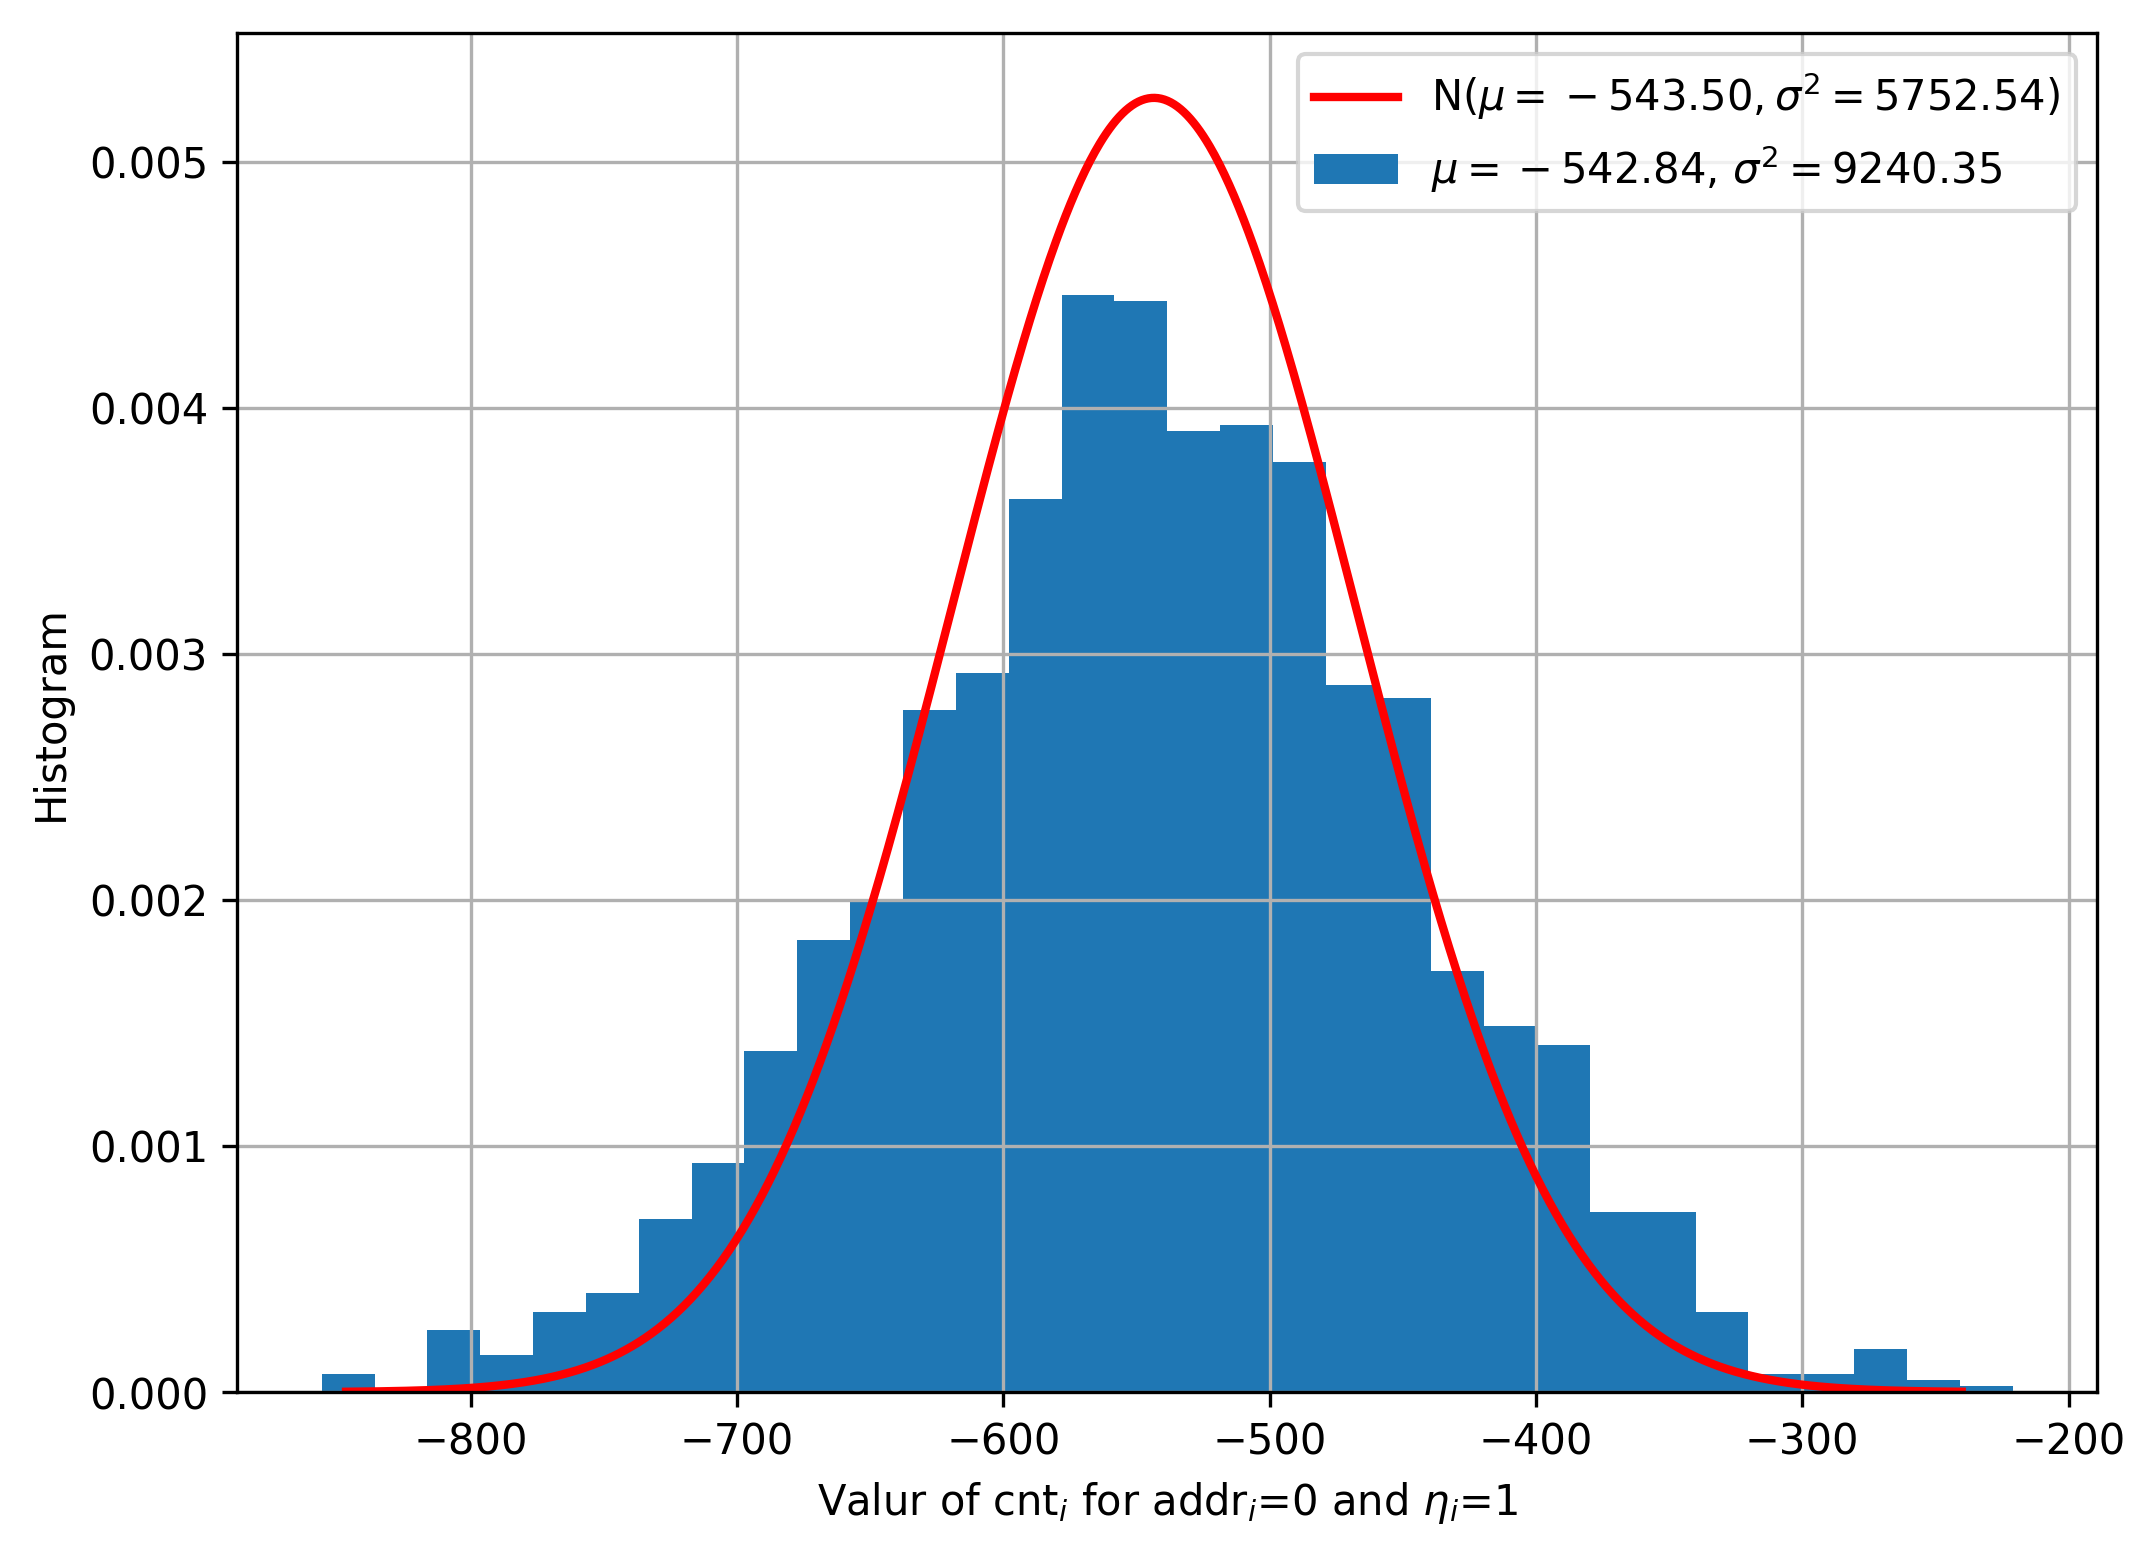
\includegraphics[width=0.5\textwidth]{./images02/autocorrelation/read-counters-eta1_addr0.png}}

  \caption{The histogram was obtained through simulation. The red curve is the theoretical normal distribution.}
  \label{fig:sdm-read-sums}
\end{figure}

Hence,

\begin{align}
\left[ \text{acc}_i|\eta_i=1 \right] &\sim \mathcal{N}(\mu = (2p-1)^2 \mu_\theta \mu_h, \sigma^2 = \sigma_\text{cnt}^2 \mu_h + 2 \mu_\text{cnt}^2 \sigma^2_h) \label{eqn:sdm-eta1} \\
\left[ \text{acc}_i|\eta_i=0 \right] &\sim \mathcal{N}(\mu = -(2p-1)^2 \mu_\theta \mu_h, \sigma^2 = \sigma_\text{cnt}^2 \mu_h + 2 \mu_\text{cnt}^2 \sigma^2_h) \label{eqn:sdm-eta0}
\end{align}

In our case, $\left[ \text{acc}_i|\eta_i=1 \right] \sim \mathcal{N}(\mu = 128.62, \sigma^2 = 12865.69)$, and $\left[ \text{acc}_i|\eta_i=0 \right] \sim \mathcal{N}(\mu = -128.62, \sigma^2 = 12865.69)$. See Figure \ref{fig:sdm-read} --- we can notice that the variance issue from Figure \ref{fig:sdm-read-sums} has propagated to these images.

\begin{figure}[h!]
  \centering
  \subfloat[Equation \ref{eqn:sdm-eta1}  ($\eta_k=1)$]{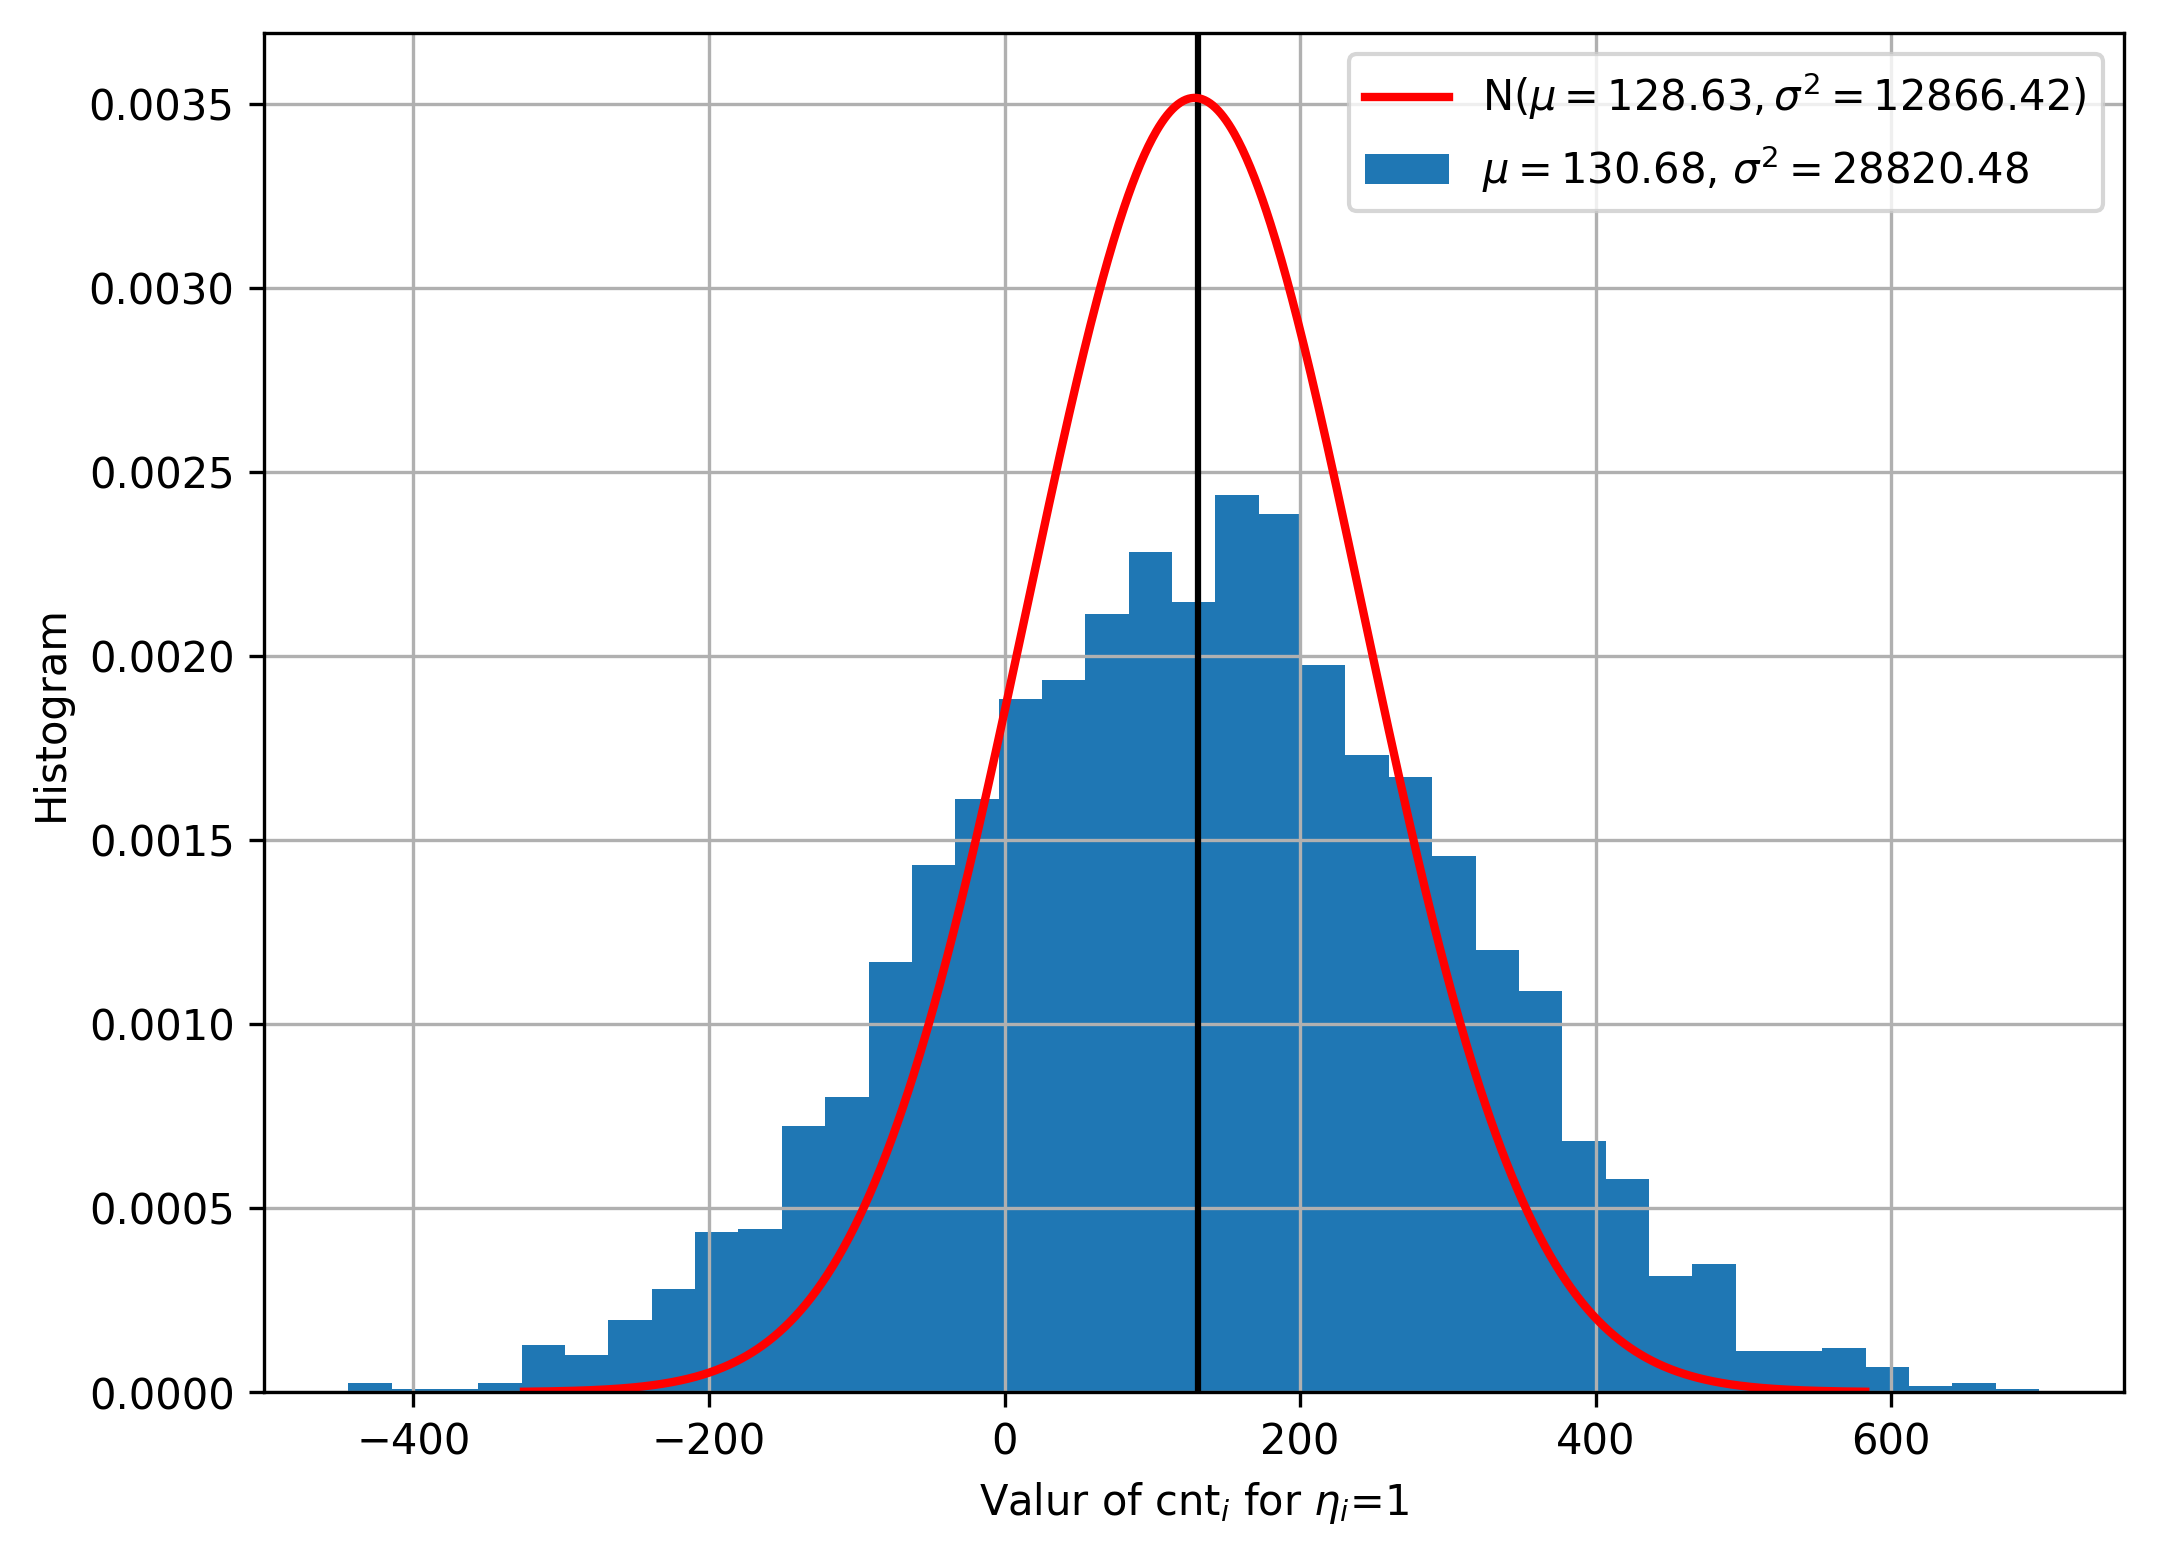
\includegraphics[width=0.5\textwidth]{./images02/autocorrelation/read-counters-eta1.png}}
  \subfloat[Equation \ref{eqn:sdm-eta0} ($\eta_k=0$)]{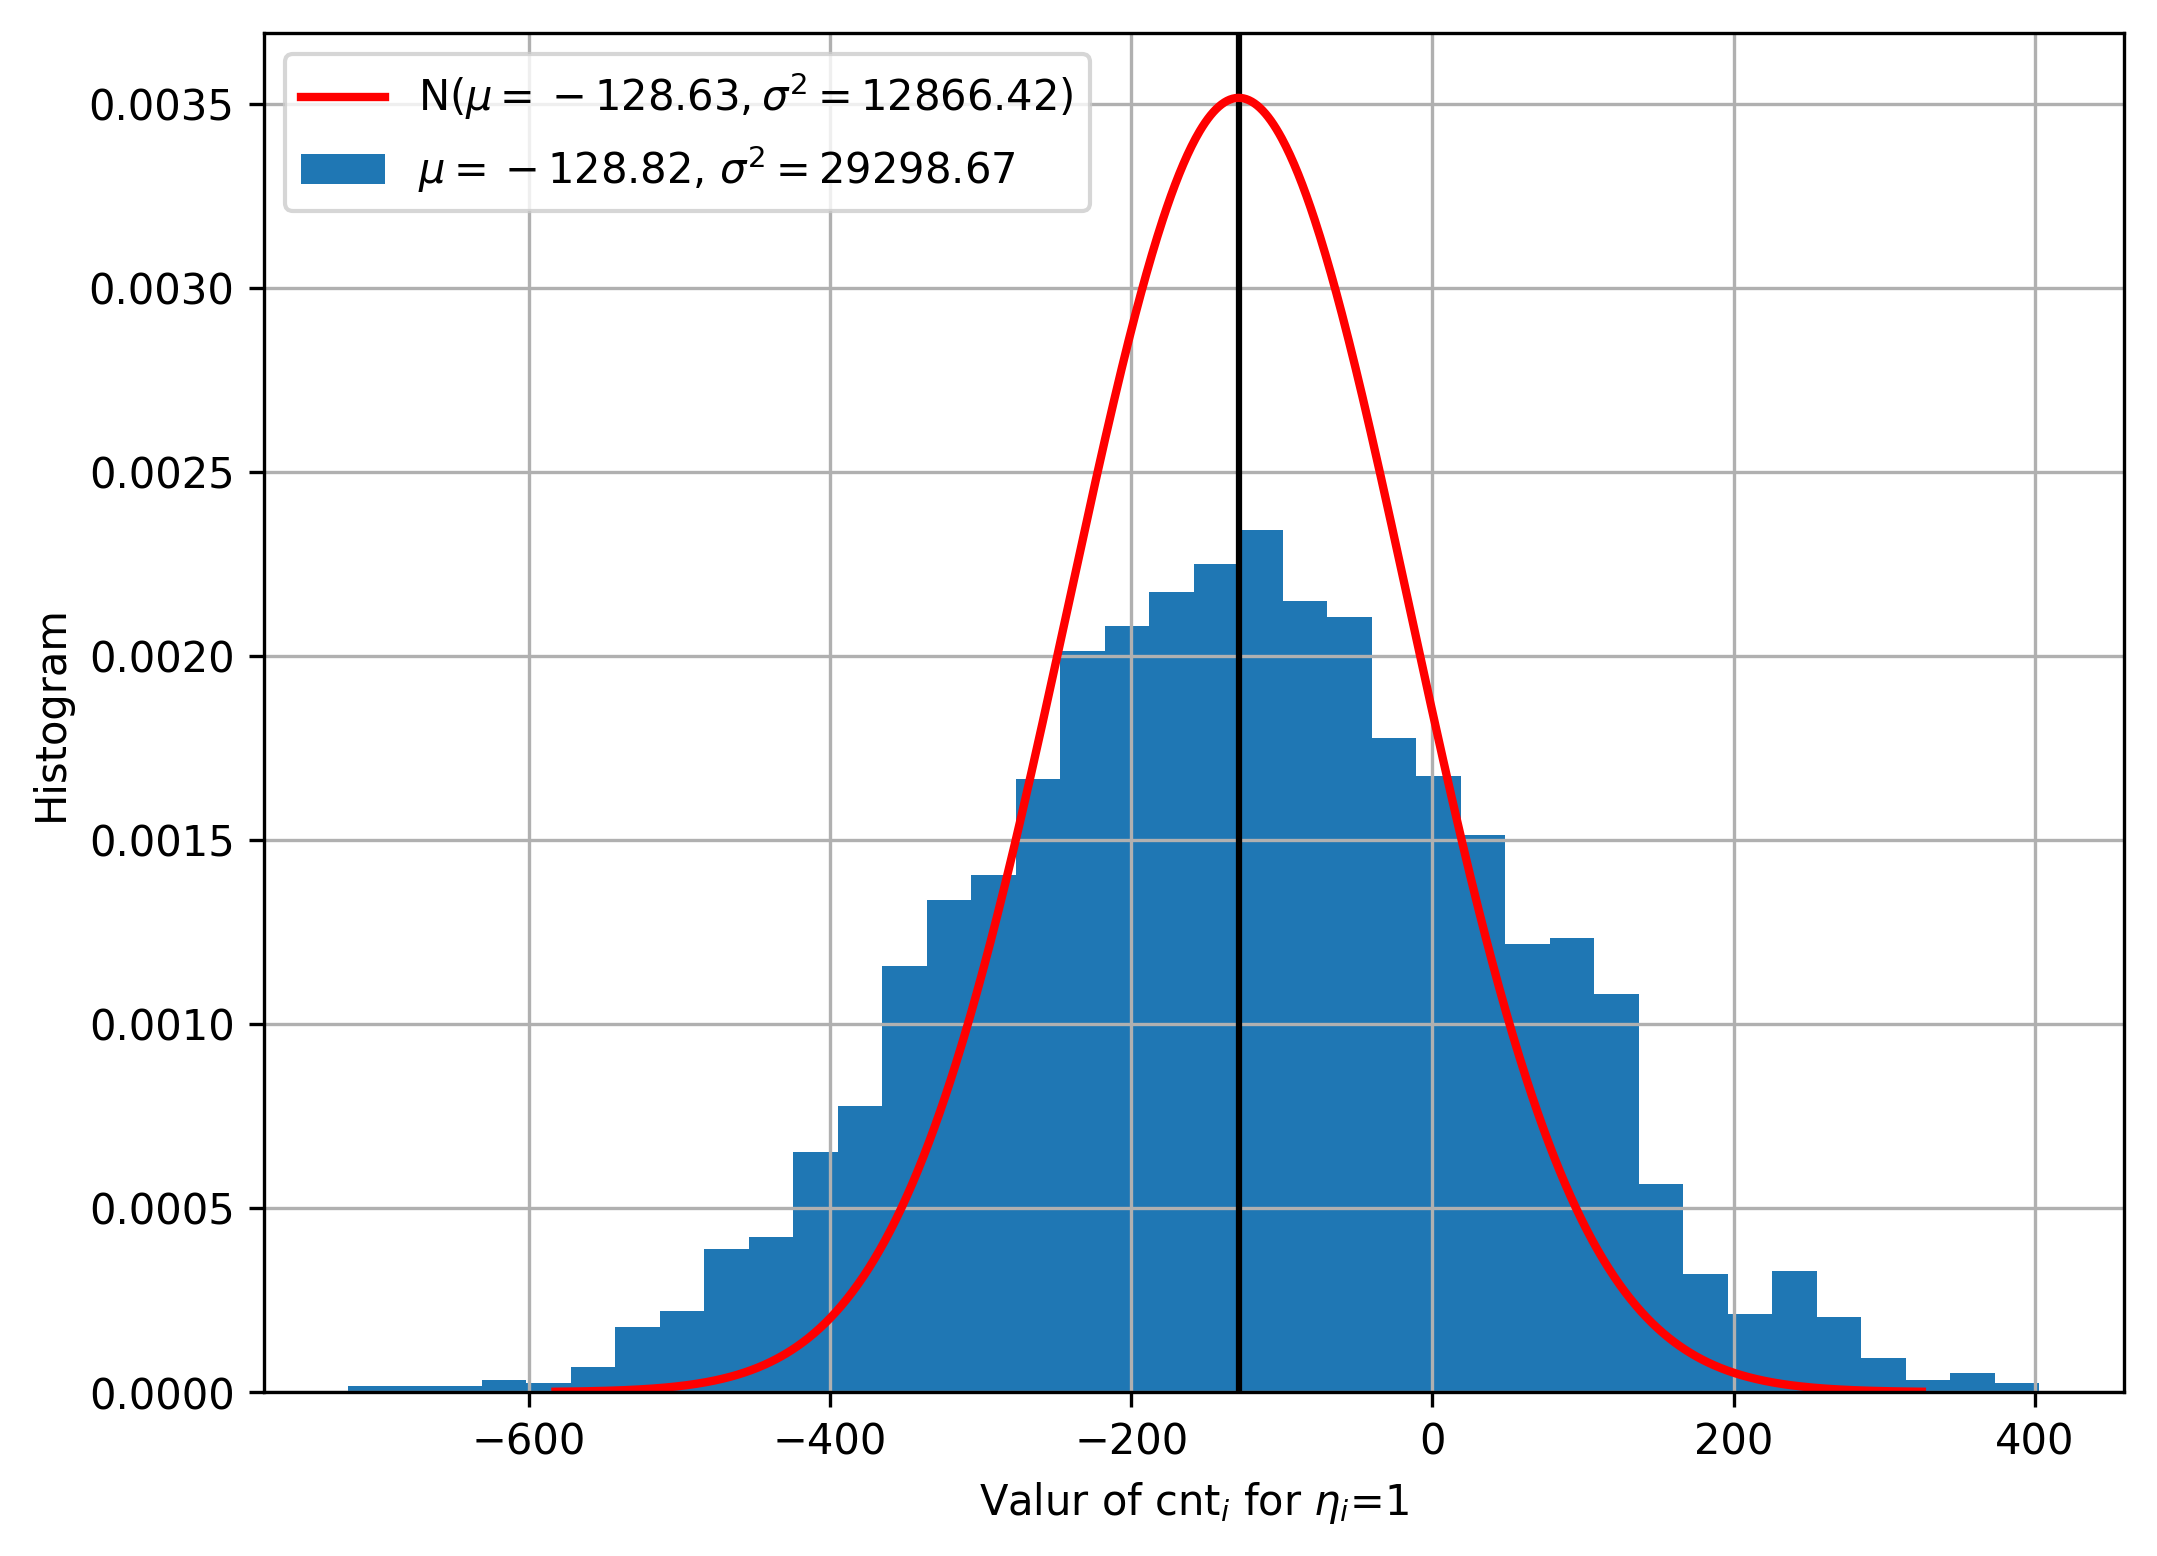
\includegraphics[width=0.5\textwidth]{./images02/autocorrelation/read-counters-eta0.png}}

  \caption{The histogram was obtained through simulation. The red curve is the theoretical normal distribution.}
  \label{fig:sdm-read}
\end{figure}


Finally,

\begin{align}
P(wrong) &= P(\text{acc}_i < 0 | \eta_i = 1) \cdot P(\eta_i = 1) + P(\text{acc}_i > 0 | \eta_i = 0) \cdot P(\eta_i = 0) \\
    &= \frac{\mathcal{N}_{\eta_i=1}.\text{cdf}(0)}{2} + \frac{1-\mathcal{N}_{\eta_i=0}.\text{cdf}(0)}{2} \\
    &= \frac{\mathcal{N}_{\eta_i=1}.\text{cdf}(0)}{2} + \frac{\mathcal{N}_{\eta_i=1}.\text{cdf}(0)}{2} \\
    &= \mathcal{N}_{\eta_i=1}.\text{cdf}(0)
\end{align}

Using the empirical variance of $\sigma^2 = 27838.3029124$, we calculate $P(wrong) = 0.22037771219874325$.

In order to check this probability, I have run a simulation reading from 1,000 random bitstrings (which have never been written into memory) and calculate the distance from the result of a single read. As the $P(wrong) = 0.22037$, I expected to get an average distance of 220.37 with a standard deviation of 13.10. See Figure \ref{fig:sdm-read-random-bs} for the comparison between the simulated and the theoretical outcomes.

Figure \ref{fig:sdm-single-read-dist} shows the new distance between $\eta_d$ and $\text{read}(\eta_d)$, where $\eta_d$ is $d$ bits away from $\eta$. As for $d \ge 520$ there is no intersection between $\eta$ and $\eta_d$, our models applies and explains the horizontal line around distance 220.

\begin{figure}[!htb]
  \centering
  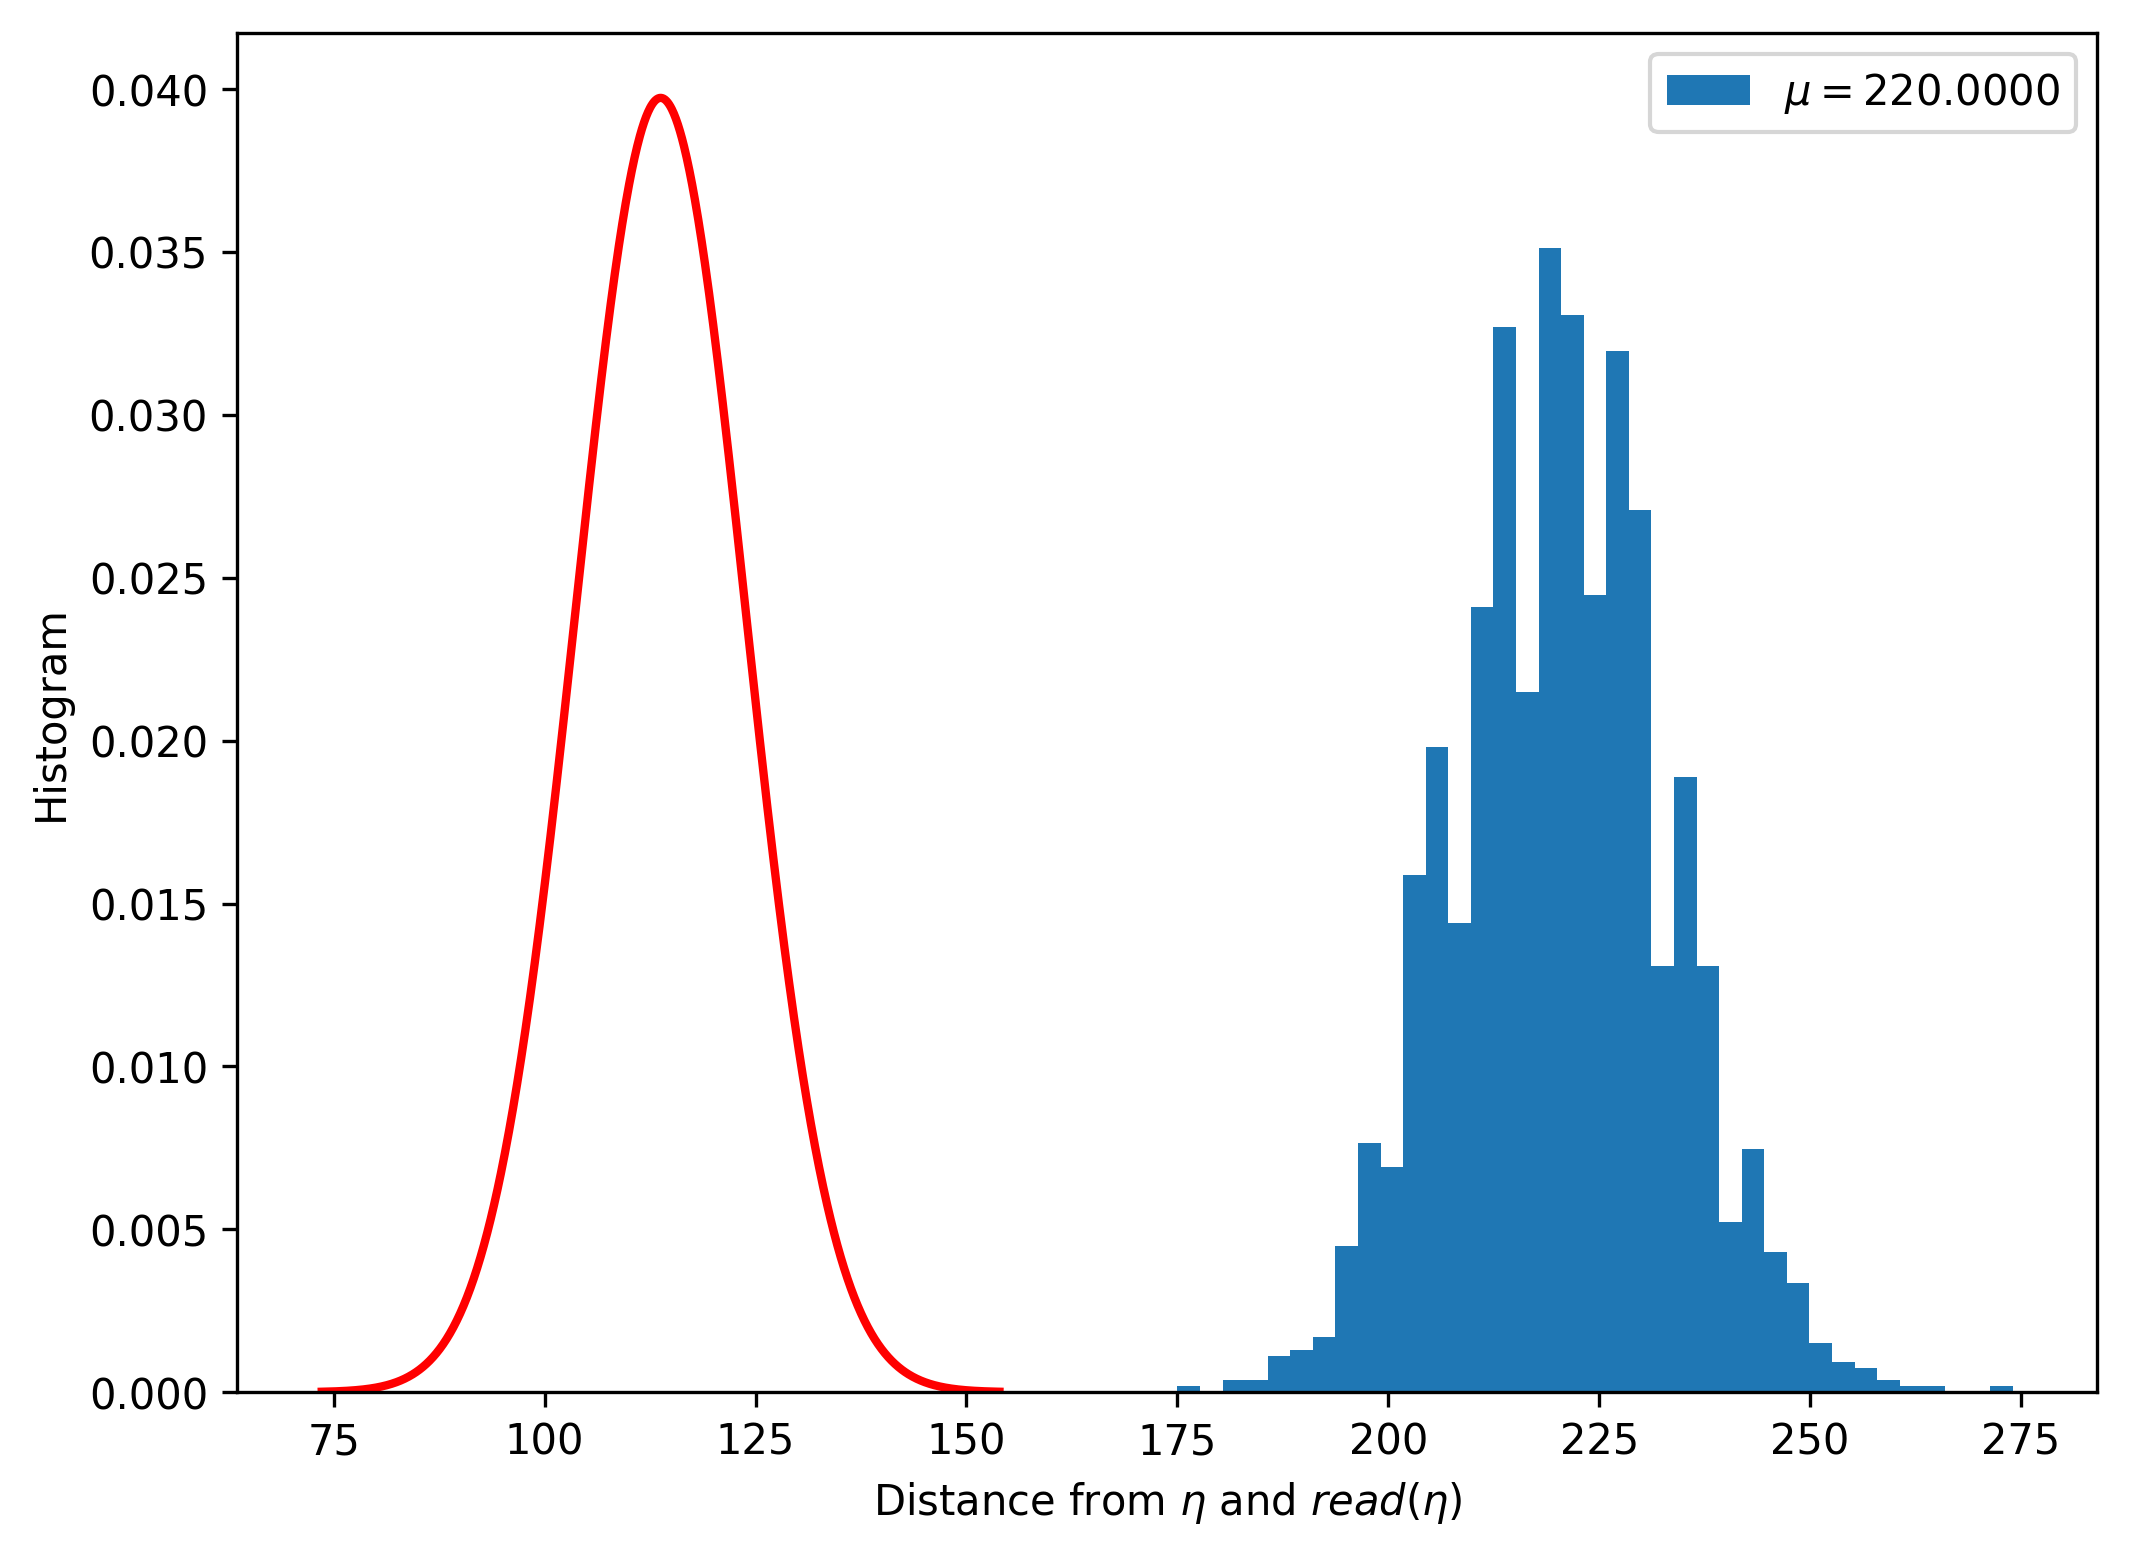
\includegraphics[width=0.6\textwidth]{./images02/autocorrelation/read-random-bs.png}

  \caption{The histogram was obtained through simulation. The red curve is the theoretical normal distribution.}
  \label{fig:sdm-read-random-bs}
\end{figure}

\begin{figure}[!htb]
  \centering
  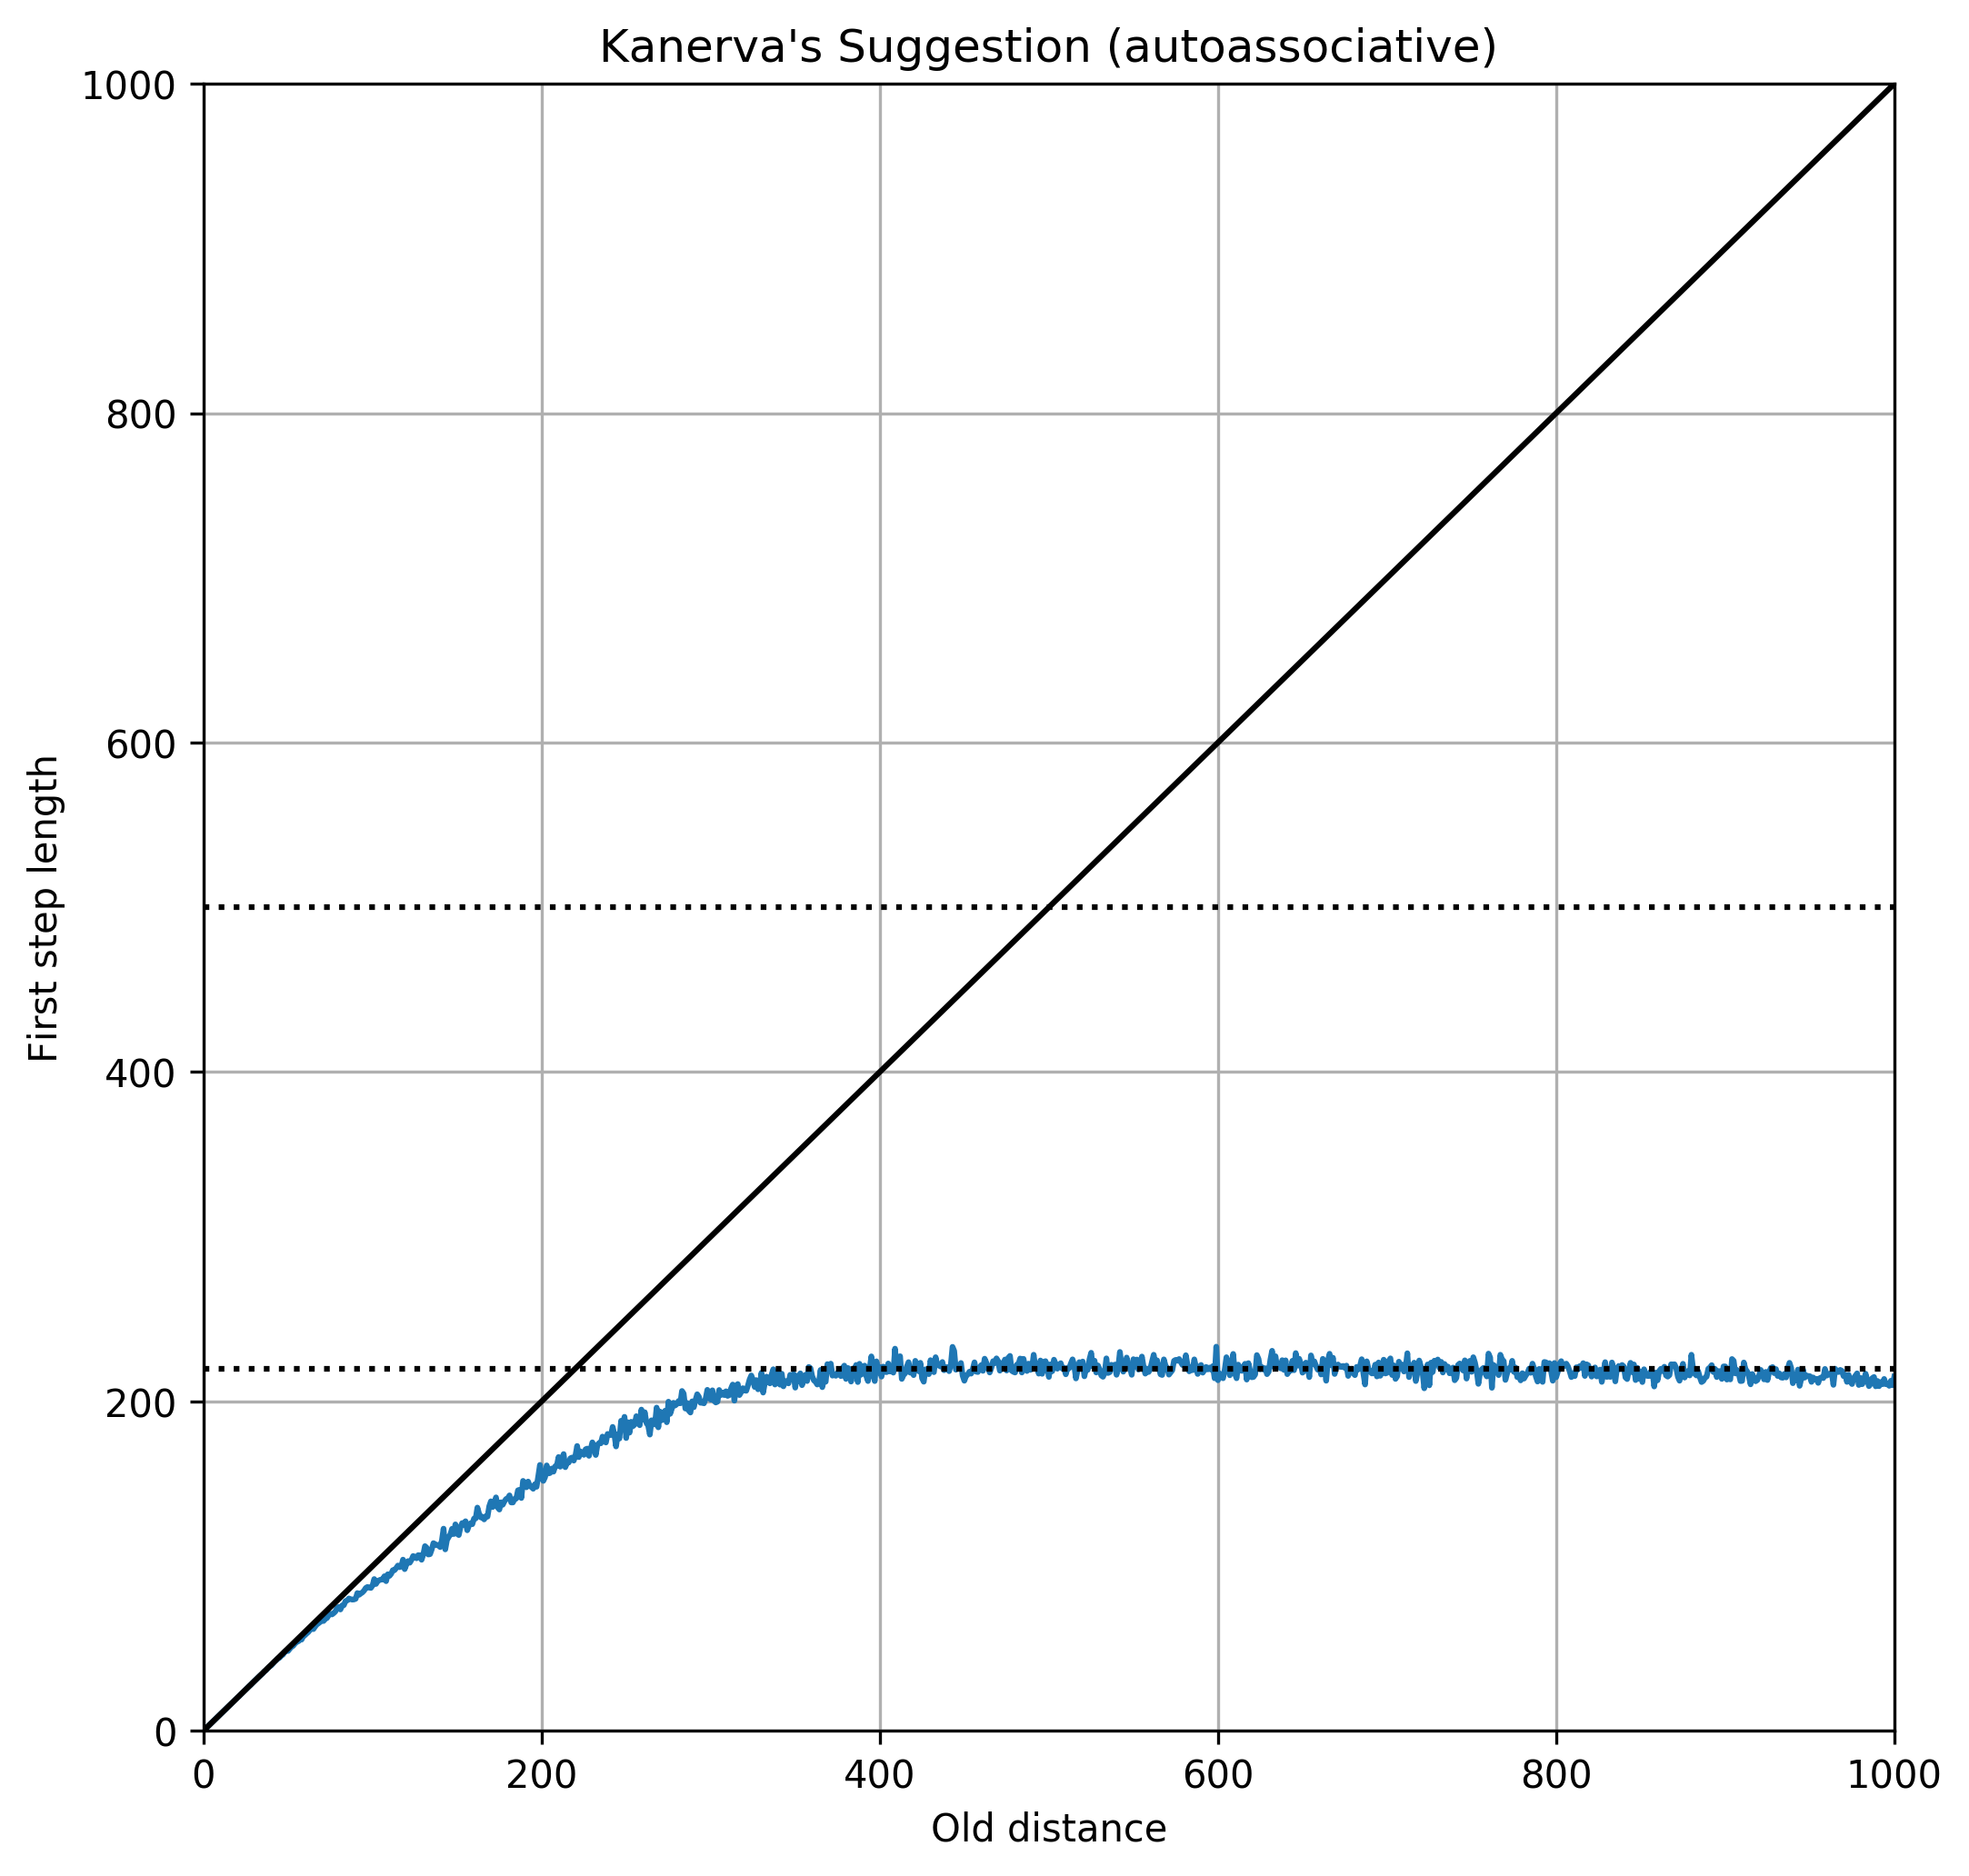
\includegraphics[width=0.6\textwidth]{./images02/autocorrelation/single-read-dist.png}

  \caption{New distance after a single read operation in a bitstring $\eta_d$, which is $d$ bits away from $\eta$. The new distance was calculated between $\eta_d$ and $\text{read}(\eta_d)$. Notice that when $d \ge 520$, the intersection between $\eta$ and $\eta_d$ is zero, which means there is only random bitstrings written into the activated hard locations. The distance 220 equals $1000 \cdot 0.220$ which is the probability find in Figure \ref{fig:sdm-read-random-bs}.}
  \label{fig:sdm-single-read-dist}
\end{figure}


\section{Conclusion}

\subsection{Effects on system-wide properties}
The skeptical reader may ask: `Beyond theory; what are the consequences of this work?  How does it apply, if at all, to building systems that incorporate SDM?'

Our conclusion is that this work is of special relevance as it brings about some \emph{systemwide properties} that models need to take into account.  The first decision choice involved in building a system with SDM regards the size of $n$, the number of dimensions of the memory.  Here, complementing the work of XXXXXXXX\footnote{check this}, we show that as $n$ grows, autocorrelation tends to $0$.  But recall that as $n$ grows, the size of the critical distance also tends to $0$.  It is therefore crucial to select a value for $n$ in which the model will retain its convergence properties, with the understanding of the possible effects brought about by autocorrelation.   Systemwide properties such as these affect the entire behavior of the model and, as such, should always be taken into account by theoreticians and modelers alike.

\subsection{Future Research}

BPs, System1 vs System2, HRRs, etc.

\subsection{Availability of the Code}

OpenCL for the partial binomail sum (cite `Inference-Based Similarity Search in Randomized Montgomery Domains for Privacy-Preserving Biometric Identification')
python (show example with figure)
Technical Documentation

Open-source Book

another article with a larger overview of the developed system so far (Reinforcement learning, critical distance, noise filtering and prototype theory, and pattern recognition.)
This --> transparency --> replicability -> incremental improvement --> parallel explorations by different teams around the world.

\section*{Acknowlegment}

The authors would like to thank Pentti Kanerva, Eric Paul Nichols, José Ricardo de Almeida Torreão, Moacyr Alvim Horta Barbosa da Silva, Flavio Codeço Coelho and Paulo Murilo Castro de Oliveira for their careful, comprehensive, reviews of the first author\textquoteright s theses.

\bibliographystyle{plain}
\bibliography{mybib02}




\begin{IEEEbiography}[{\fbox{\begin{minipage}[t][1.25in]{1in}%
Replace this box by an image with a width of 1\,in and a height of
1.25\,in!%
\end{minipage}}}]{Marcelo Salhab Brogliato} received the Ph.D. degree from Getulio Vargas Foundation in 2018. Vialink, sdm.ai,
\end{IEEEbiography}




%\begin{IEEEbiography}[{\fbox{\begin{minipage}[t][1.25in]{1in}{Linhares.jpg}

\begin{IEEEbiography}[
  {
  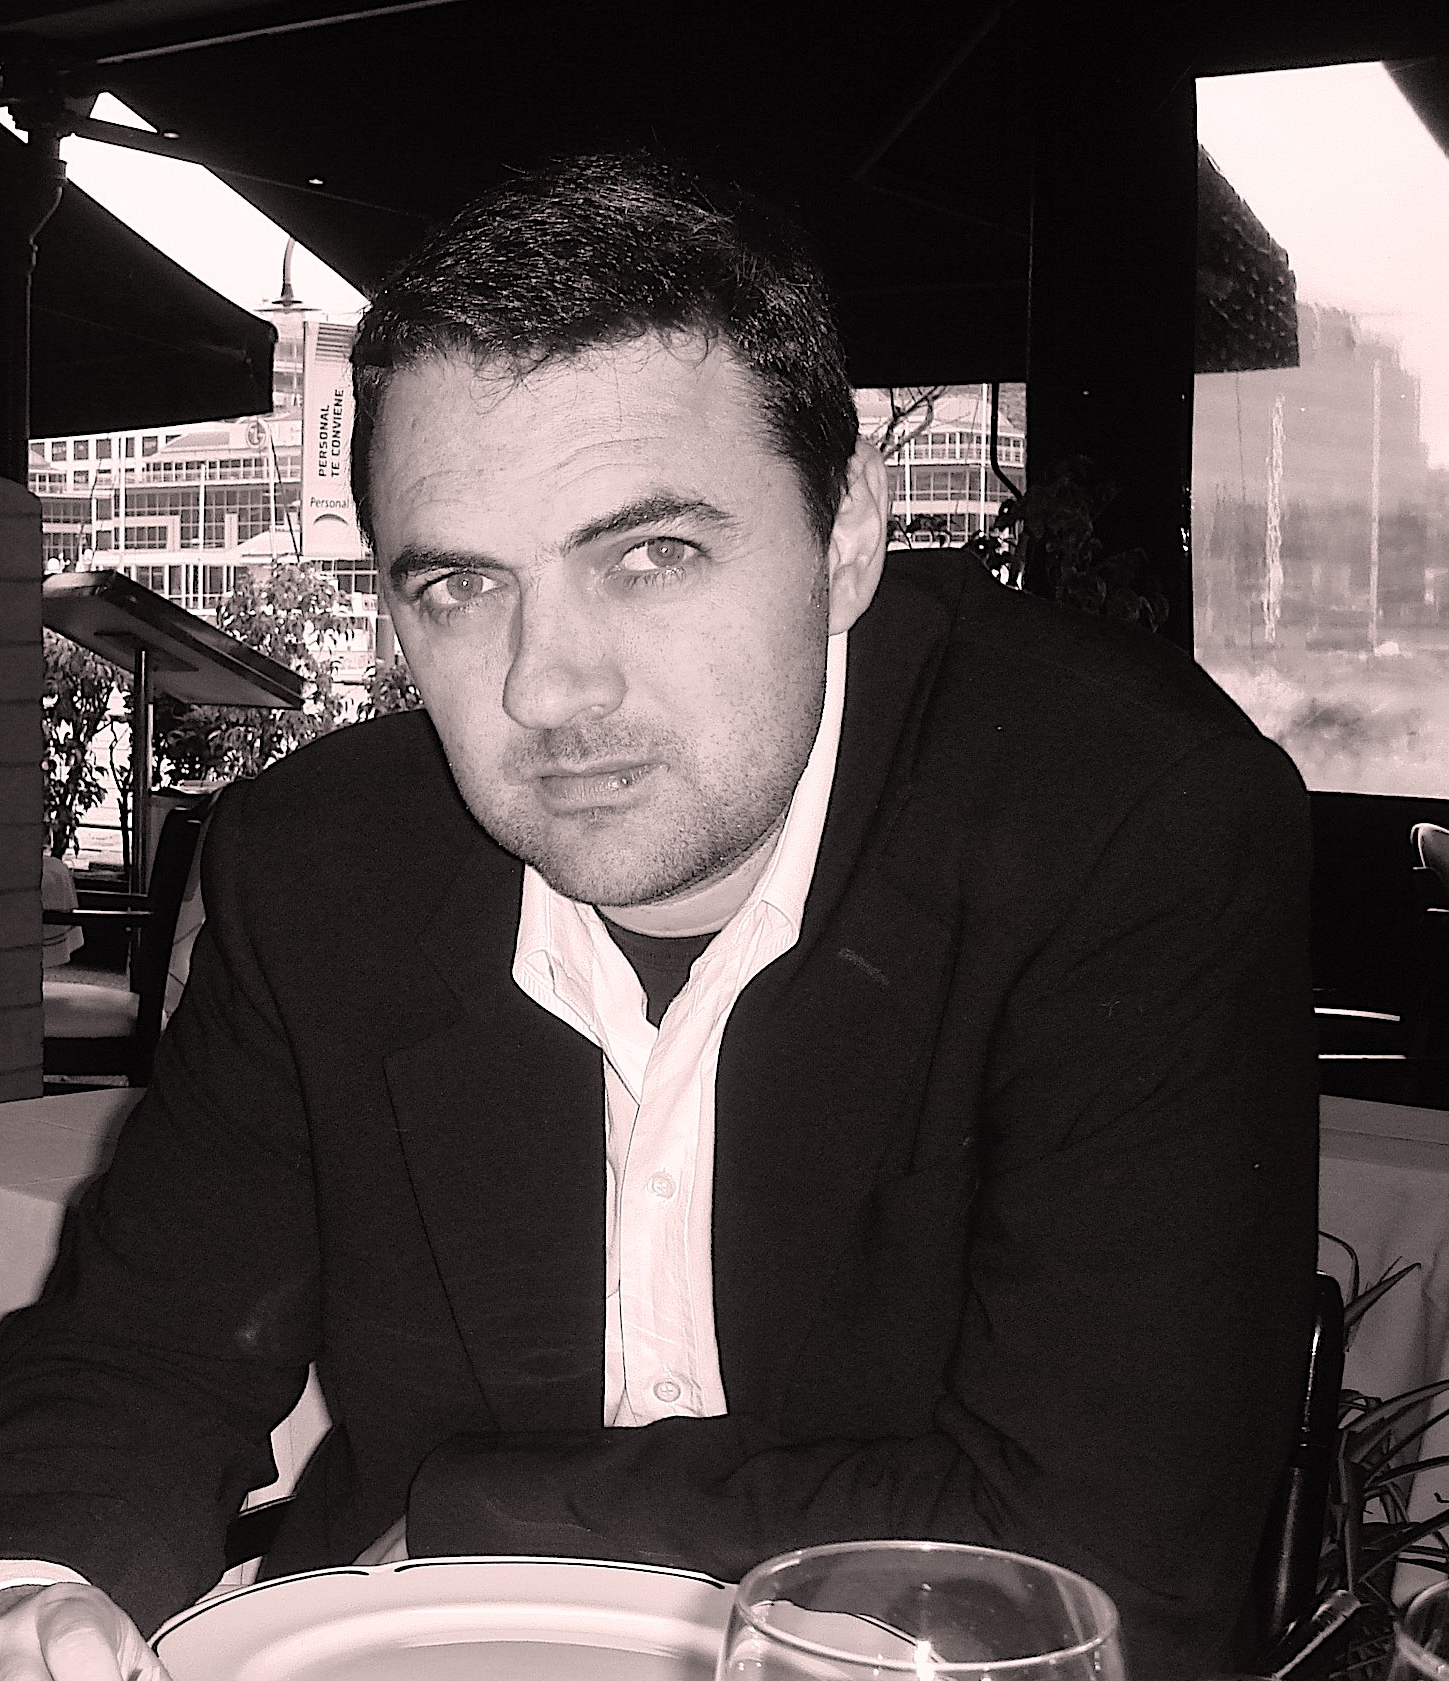
\includegraphics[width=1in,height=1.25in,clip]{./Chapters/Linhares.jpg}
  }
  ]
{Alexandre Linhares} received the Ph.D. degree from the National Institute of Space Research, 2001. He is an Associate Professor at the Center of Behavioral Research, EBAPE / Getulio Vargas Foundation.  He has published ~30 papers in journals such as \emph{Artificial Intelligence, Applied Intelligence, Biological Cybernetics, Cognitive Science, Cognitive Systems Research, Computers & Operations Research, IEEE Transactions on Evolutionary Computation, Information Sciences, Frontiers in Human Neuroscience,} among others.
\end{IEEEbiography}


\end{document}
